\chapter{Diseño del proyecto}\label{cap3}
Conforme a lo visto en el Capítulo \ref{cap2}, el proyecto AutoSA requiere ser ejecutado de dos formas distintas:
\begin{enumerate}
 	\item Rutinas automatizadas: se ejecutan a partir del entorno gráfico del sistema operativo.
 	\item Portal de usuario: se ofrece como una página web, la cual depende del servidor web de la farmacéutica y del explorador web del usuario.
\end{enumerate}
Por otro lado, es necesario contar con una base de datos, la cual debe mantener los datos de las órdenes de reposición persistentes. También es necesario mantener el acceso al sistema de archivos para guardar las capturas de pantalla de las órdenes de reposición enviadas. Por lo que es necesario tener dos ambientes de ejecución: la automatización, que será ejecutada exclusivamente en el sistema operativo, y la web, que se ejecuta en el sistema operativo y en el explorador de internet del usuario.


%===============================================================================
%===============================================================================


\section{Diseño de la arquitectura del sistema AutoSA}
Bourque\cite{SWEBOOK} define la arquitectura de software como:
\begin{quote}
	El conjunto de estructuras necesarias para la comprensión de un sistema en el cual se comprometen elementos de software, relaciones entre ellos y sus propiedades.
\end{quote}
En las últimas décadas la arquitectura de software ha profundizado en el estudio genérico de las estructuras del software, lo que ha dado lugar a técnicas como los patrones de diseño (Apéndice \ref{sec:patrones}) \cite{SWEBOOK, SoftwareArchitectureInAction}.

\subsection{Arquitectura en capas}
Un tipo de arquitectura es la arquitectura en capas que Richards\cite{SoftwareArchitecturePatterns} describe como:
\begin{quote}
La arquitectura en capas, conocida también como arquitectura de n-niveles, consiste de componentes organizados en capas horizontales, donde cada capa tiene un rol específico dentro de la aplicación. Una de las propiedades más poderosas de la arquitectura en capas es la separación de responsabilidades entre componentes, es decir, componentes dentro de una misma capa se encargan de la lógica que atañe a dicha capa.
\end{quote}

El sistema AutoSA consta de dos aplicaciones, una aplicación de escritorio encargada de ejecutar las rutinas de automatización y una aplicación web encargada de ofrecer operaciones de administración sobre las órdenes de reposición atendidas.\\
En la Figura \ref{fig:dia-layers-auto} se muestra el diagrama de la arquitectura en capas de la aplicación de escritorio, mientras que en la Figura \ref{fig:dia-layers-web} se encuentra el diagrama de la arquitectura en capas de la aplicación web. Ambas arquitecturas constan de las siguientes capas:
\begin{enumerate}
	\item Presentación: tiene la responsabilidad de la interfaz de usuario.
	\item Lógica de negocio: contiene los componentes que implementan las reglas del negocio.
	\item Servicios: contiene los servicios encargados del acceso a recursos compartidos.
	\item Acceso a datos: está formado por los componentes que proveen acceso a la lectura y escritura de datos.
	\item Datos: son los recursos encargados de contener la información persistente del sistema.
\end{enumerate}

%espaciado
\pagebreak
%espaciado

\begin{figure}[h]
\centering
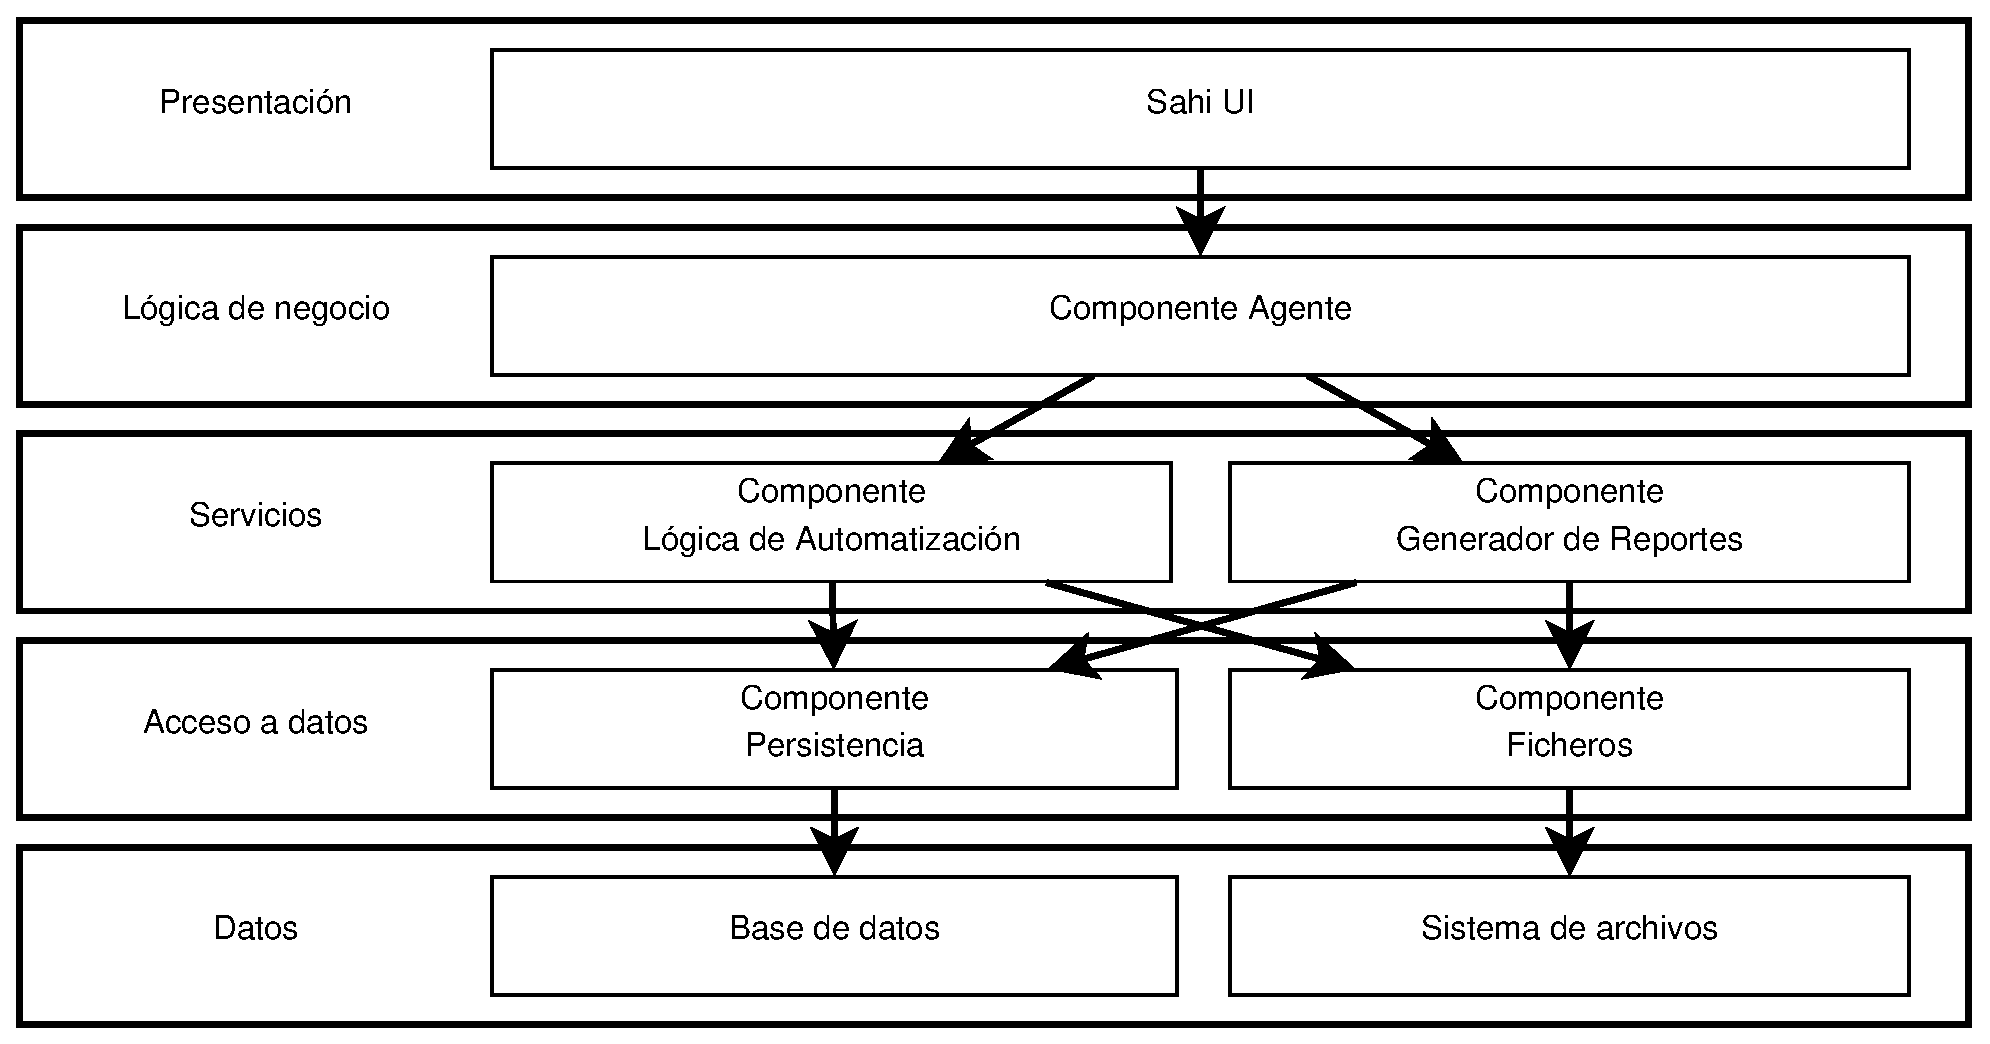
\includegraphics[scale=0.4]{dia-layers-auto}
\caption{Diagrama en capas de la aplicación de escritorio.}
\label{fig:dia-layers-auto}
\end{figure}

\begin{figure}[h]
\centering
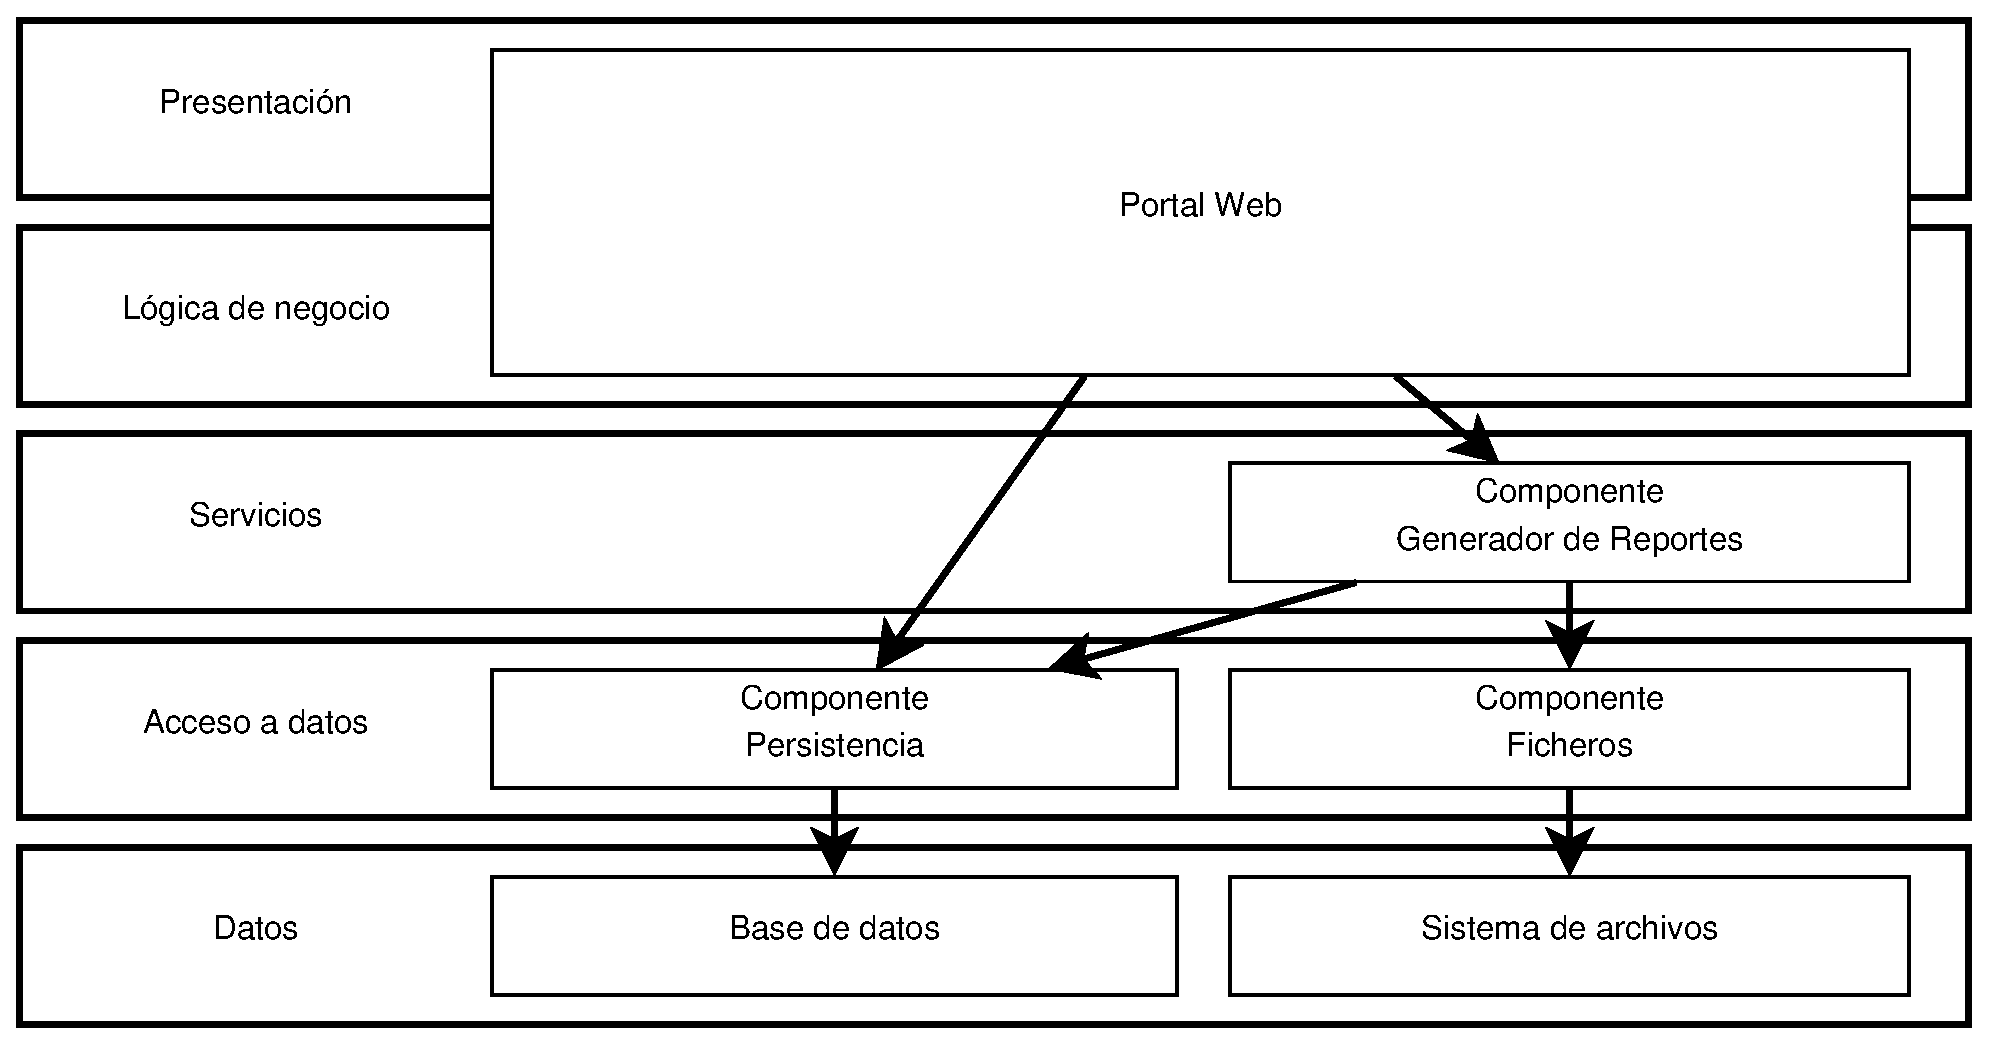
\includegraphics[scale=0.4]{dia-layers-web}
\caption{Diagrama en capas de la aplicación web.}
\label{fig:dia-layers-web}
\end{figure}

%Siguiendo el concepto de arquitectura, se muestran los componentes del sistema y su respectiva solución a los casos de uso del Capítulo \ref{sec:casos-uso}.

\subsection{Componentes del sistema AutoSA}
El diagrama de componentes sirve para visualizar los componentes en los que se divide el sistema y las interfaces por las cuales se comunican tales componentes. El la Figura \ref{fig:dia-components} se muestra el diagrama de componentes para el sistema AutoSA. En las secciones subsecuentes se describe cada componente y las interfaces que ofrece\footnote{Únicamente se mostrarán los diagramas de secuencia más completos que reflejan un comportamiento no trivial.}.
\begin{figure}[h]
\centering
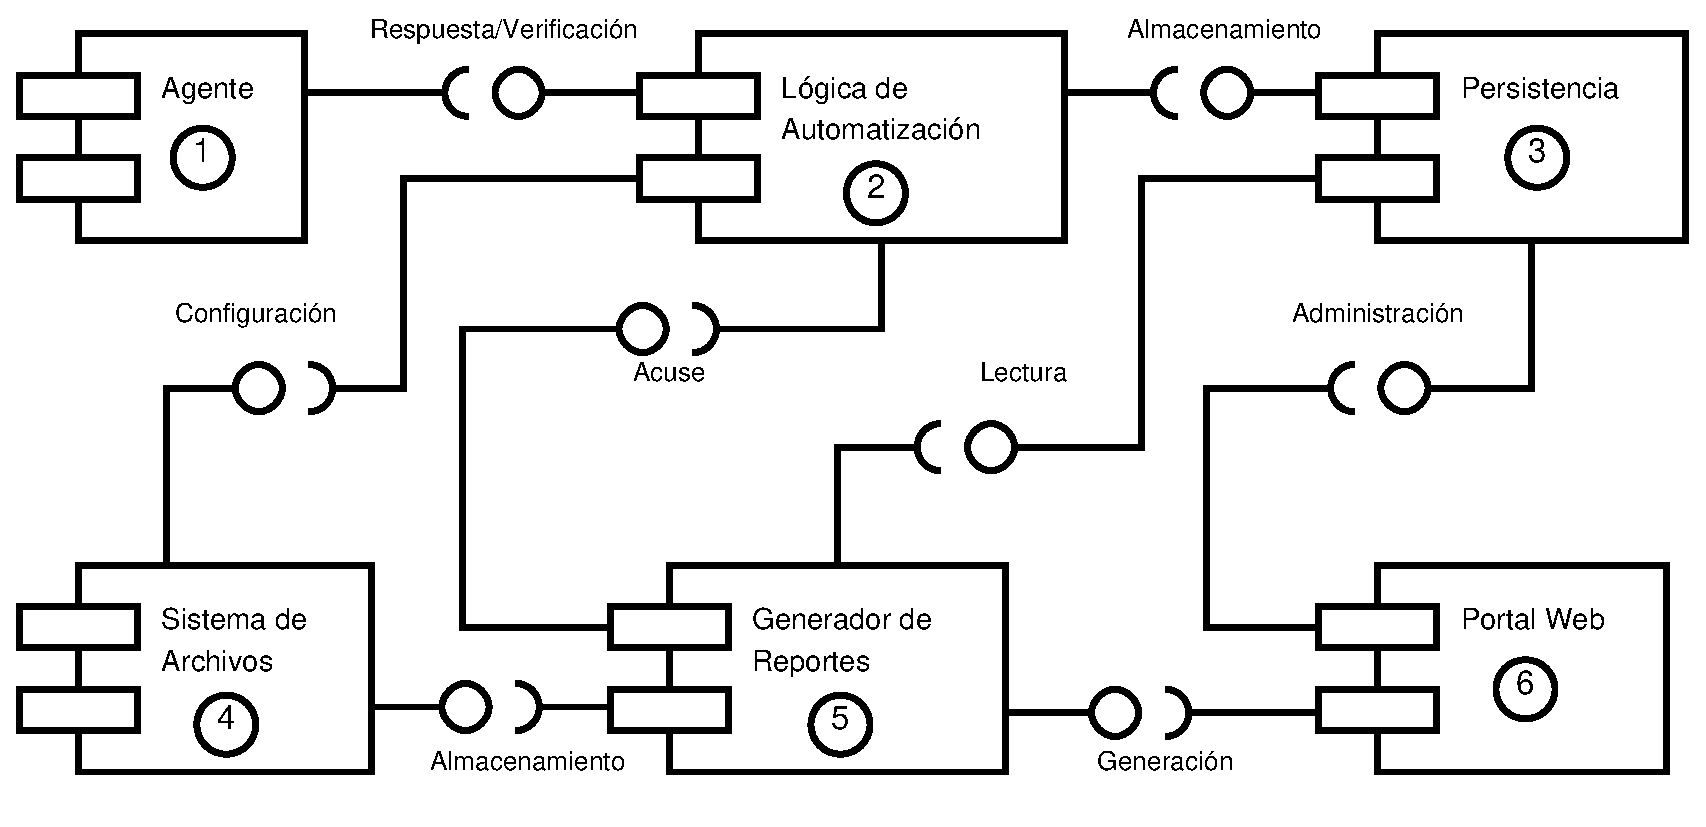
\includegraphics[width=\textwidth]{dia-components}
\caption{Diagrama de componentes.}
\label{fig:dia-components}
\end{figure}

\subsubsection{Agente}
El componente que contiene y ejecuta las rutinas de automatización, esto es mediante una interfaz con el usuario en la cual puede seleccionar el proceso a ser ejecutado. No ofrece interfaces a los demás componentes, consume exclusivamente el componente \textbf{Lógica de Automatización}.

\subsubsection{Lógica de Automatización}\label{sec:logica-auto}
La función de este componente es ejecutar las reglas de negocio necesarias en los flujos de los procesos de automatización. Ofrece las interfaces de respuesta y verificación.
\paragraph{\indent Interfaz Respuesta\\}
Provee el acceso a las reglas de negocio del proceso de respuesta de órdenes de reposición (caso de uso \textbf{CU-CONTESTAR}). Esta interfaz expone las siguientes operaciones:
\begin{enumerate}
	\item \textbf{guardar-orden-nueva}: guarda un listado de nuevas órdenes de reposición.
	\item \textbf{obtener-orden-contestar}: da la siguiente orden de reposición para contestar.
	\item \textbf{obtener-datos-respuesta}: da los datos necesarios para llenar los formularios para contestar una orden de reposición en el \textit{Sistema de Abastecimiento}.
	\item \textbf{actualizar-orden-contestada}: actualiza los datos almacenados de la orden de reposición con los datos de la respuesta en el \textit{Sistema de Abastecimiento}. Utiliza el componente \textbf{Persistencia} para actualizar los datos.
	\item \textbf{obtener-orden-enviar}: da la siguiente orden de reposición para enviar.
	\item \textbf{guardar-orden-enviada}: actualiza los datos almacenados de la orden de reposición con los datos de la pantalla de envío del \textit{Sistema de Abastecimiento}. Utiliza el componente \textbf{Persistencia} para actualizar los datos.
	\item \textbf{obtener-acuse-envio}: solicita la generación de el acuse de envío al componente de reportes y almacena el documento por medio del componente \textbf{Ficheros}.
\end{enumerate}

\paragraph{\indent Interfaz Verificación\\}
Provee el acceso a las reglas de negocio del proceso de verificación de órdenes de reposición canceladas. Esta interfaz expone las siguientes operaciones:
\begin{enumerate}
	\item \textbf{obtener-rango-verificar}: obtiene el rango de fechas para ingresar en el formulario de búsqueda del \textit{Sistema de Abastecimiento}. El número de días que comprende el rango se obtiene utilizando el componente \textbf{Ficheros}.
	\item \textbf{actualizar-estado-sa}: actualiza el EstadoSA de las órdenes de reposición recibidas a \textbf{Cancelada}. Utiliza el componente \textbf{Persistencia} para la actualización de datos.
\end{enumerate}

\subsubsection{Persistencia}
Este componente está encargado de las operaciones de persistencia hacia la base de datos, su diseño está basado en el Patrón DAO (Apéndice \ref{sec:dao}) para controlar el acceso a la base de datos\footnote{En adelante se utilizará DAO para hacer referencia al patrón y la instancia (objeto) del patrón.}.\\
El componente \textbf{Persistencia} del proyecto AutoSA presenta las siguientes interfaces de búsqueda y almacenamiento:

\paragraph{\indent Interfaz Almacenamiento\\}
Conjunto de operaciones diseñadas para responder a las necesidades de almacenamiento en los flujos para responder y verificar órdenes de reposición\footnote{Casos de uso CU-CONTESTAR, CU-GUARDAR-NUEVA, CU-RESPONDER-ORDEN, CU-ENVIAR-ORDEN y CU-ACTUALIZAR-ESTATUS-SA.}. Esta interfaz expone las siguientes operaciones:
\begin{enumerate}
	\item \textbf{guardar-nueva}: inserta una nueva orden de reposición en la base de datos.
	\item \textbf{cambiar-estado}: cambia el estado de atención de una orden de reposición.
	\item \textbf{guardar-respuesta}: guarda los datos de los formularios de la pantalla de respuesta de las órdenes de reposición.
	\item \textbf{guardar-folio-acuse}: guarda el folio de acuse de envío de la orden de reposición.
	\item \textbf{actualizar-estado-sa}: actualiza el estado de atención en el \textit{Sistema de Abastecimiento} a \textbf{cancelada} de las órdenes de reposición recibidas.
	\item \textbf{registrar-evento}: registra en la base de datos un evento que ocurre durante los procesos automatizados. El evento puede ser de carácter informativo o de error.
\end{enumerate}

\paragraph{\indent Interfaz Lectura\\}
Conjunto de operaciones diseñadas para las necesidades de lectura de órdenes de reposición en los flujos para responder y verificar órdenes de reposición\footnote{Ver casos de uso \textbf{CU-CONTESTAR}, \textbf{CU-ENVIAR-ORDEN} y \textbf{CU-GENERAR-ACUSE}.}. Esta interfaz expone las siguientes operaciones:
\begin{enumerate}
	\item \textbf{siguiente-orden-contestar}: entrega un mapa con los datos de la primera orden de reposición encontrada con estado \textbf{Nueva}.
	\item \textbf{siguiente-orden-enviar}: entrega un mapa con los datos de la primera orden de reposición encontrada con estado \textbf{Contestada}.
	\item \textbf{obtener-datos-acuse}: obtiene los datos de una orden de reposición necesarios para generar el documento de acuse de envío.
\end{enumerate}

\paragraph{\indent Interfaz Administración\\}
Son las operaciones que permiten modificar datos específicos de las órdenes de reposición contenidas en la base de datos. También ofrece la actualización masiva de catálogos\footnote{Ver casos de uso \textbf{CU-ENTRAR-WEB}, \textbf{CU-GENERAR-REPORTE}, \textbf{CU-ACTUALIZAR-CATALOGO}, \textbf{CU-BUSCAR}, \textbf{CU-VISUALIZAR} y \textbf{CU-EDITAR}.}. Esta interfaz expone las siguientes operaciones:
\begin{enumerate}
	\item \textbf{buscar-credenciales}: busca las credenciales del usuario.
	\item \textbf{extraer-reporte}: ejecuta la búsqueda necesaria para extraer los datos del reporte indicado.
	\item \textbf{actualizar-catalogo}: actualiza la información del catálogo indicado.
	\item \textbf{buscar-ordenes}: busca órdenes de reposición que cumplan con el filtro de búsqueda indicado.
	\item \textbf{buscar-orden}: busca una orden de reposición por el número de orden.
	\item \textbf{actualizar-orden}: actualiza los datos de orden de reposición.
\end{enumerate}

\subsubsection{Ficheros}
El componente \textbf{Ficheros} está encargado de la comunicación con el sistema de archivos del sistema operativo, tiene la función de realizar la lectura de archivos de configuración, el almacenamiento de los acuses de envío y los reportes de las órdenes de reposición.\\
Este componente, al igual que el componente \textbf{Persistencia}, está diseñado siguiendo el Patrón DAO.

\paragraph{\indent Interfaz Configuración\\}
Da la configuración escrita en archivos de propiedades contenidos en el mismo sistema de archivos. Esta interfaz expone las siguiente operación:

\begin{enumerate}
	\item \textbf{obtener-propiedad}: obtiene una propiedad de los archivos de configuración.
\end{enumerate}

%espaciado
\pagebreak
%espaciado

\paragraph{\indent Interfaz Almacenamiento\\}
Almacena archivos (reportes y acuses de envío) en el sistema de archivos. Esta interfaz expone las siguiente operación:
\begin{enumerate}
	\item \textbf{guardar-archivo}: guarda un archivo en el sistema de archivos.
\end{enumerate}

\subsubsection{Generador de Reportes}
El generador de reportes, como su nombre lo indica, tiene la función de generar documentos y reportes con los datos de las órdenes de reposición almacenados en la base de datos. 
\paragraph{\indent Interfaz Acuse\\} Genera el documento con el acuse de envío. Esta interfaz expone las siguientes operaciones:
\begin{enumerate}
	\item \textbf{generar-acuse-envio}: genera el acuse de envío para la orden de reposición especificada. Utiliza el componente \textbf{Persistencia} para obtener los datos de la orden.
\end{enumerate}

\paragraph{\indent Interfaz Generación\\} Genera reportes con los datos de las órdenes de reposición almacenados en la base de datos. Esta interfaz expone las siguientes operaciones:
\begin{enumerate}
	\item \textbf{generar-reporte-ordenes}: genera el reporte del tipo indicado usando el rango de fechas establecido.
\end{enumerate}

\subsubsection{Portal Web}
El componente que ofrece al usuario las funcionalidades de una interfaz web. Está diseñado siguiendo el Patrón MVC (sección \ref{sec:mvc}) y utiliza el componente \textbf{Persistencia} como el Modelo, mientras que la Vista se toma en dos partes: las pantallas que se muestran al usuario y los reportes. Para esta última toma las funciones del componente \textbf{Generación de Reportes} y \textbf{Ficheros}.\\
No ofrece interfaces a los demás componentes, al igual que el componente Agente.



\subsection{Solución a casos de uso}
A continuación se presentan las soluciones a los casos de uso utilizando los componentes descritos en la sección anterior. Para este fin se utilizan diagramas de secuencia UML (sección \ref{sec:uml-seq}).

\subsubsection{Contestar órdenes}
El diseño de la solución al caso de uso \textbf{CU-CONTESTAR} (sección \ref{cu-contestar}) se lleva a cabo entre el actor \textbf{Usuario} y los componentes \textbf{Agente} \textbf{Lógica de Automatización}. La solución sigue la siguiente secuencia (Figura \ref{fig:dia-seq-cu-contestar}\footnote{Por cuestión del tamaño de la figura y para conservar el texto dentro de ella de tamaño legible, únicamente se mostrarán los mensajes más importantes entre componentes.}):
\begin{enumerate}
	\item \textbf{Usuario}: inicia la ejecución del agente (mensaje 1 del diagrama de la Figura \ref{fig:dia-seq-cu-contestar}).
	\item \textbf{Agente}: dirige el explorador de internet a la página del \textit{Sistema de Abastecimiento} y solicita al usuario la contraseña para ingresar.
	\item \textbf{Usuario}: proporciona la contraseña (mensaje 2 del diagrama de la Figura \ref{fig:dia-seq-cu-contestar}).
	\item \textbf{Agente}: realiza el acceso al \textit{Sistema de Abastecimiento}.
	\item \textbf{Agente}: dirige el explorador de Internet al listado de órdenes de reposición.
	\item \textbf{Agente}: para cada orden en el listado ejecuta el caso de uso \textbf{CU-GUARDAR-NUEVA} con apoyo del componente \textbf{Lógica de Automatización} (mensaje 3 del diagrama de la Figura \ref{fig:dia-seq-cu-contestar}).
	\item \textbf{Agente}: para cada orden con estado de \textbf{NUEVA} en la base de datos ejecuta el caso de uso \textbf{CU-RESPONDER-ORDEN} con apoyo del componente \textbf{Lógica de Automatización} (mensaje 4 del diagrama de la Figura \ref{fig:dia-seq-cu-contestar}).
	\item \textbf{Agente}: para cada orden con estado de \textbf{CONTESTADA} en la base de datos, ejecuta los casos de uso \textbf{CU-ENVIAR-ORDEN} y \textbf{CU-GENERAR-ACUSE} con apoyo del componente \textbf{Lógica de Automatización} (mensaje 5 del diagrama de la Figura \ref{fig:dia-seq-cu-contestar}).
\end{enumerate}

\begin{figure}[h]
	\centering
	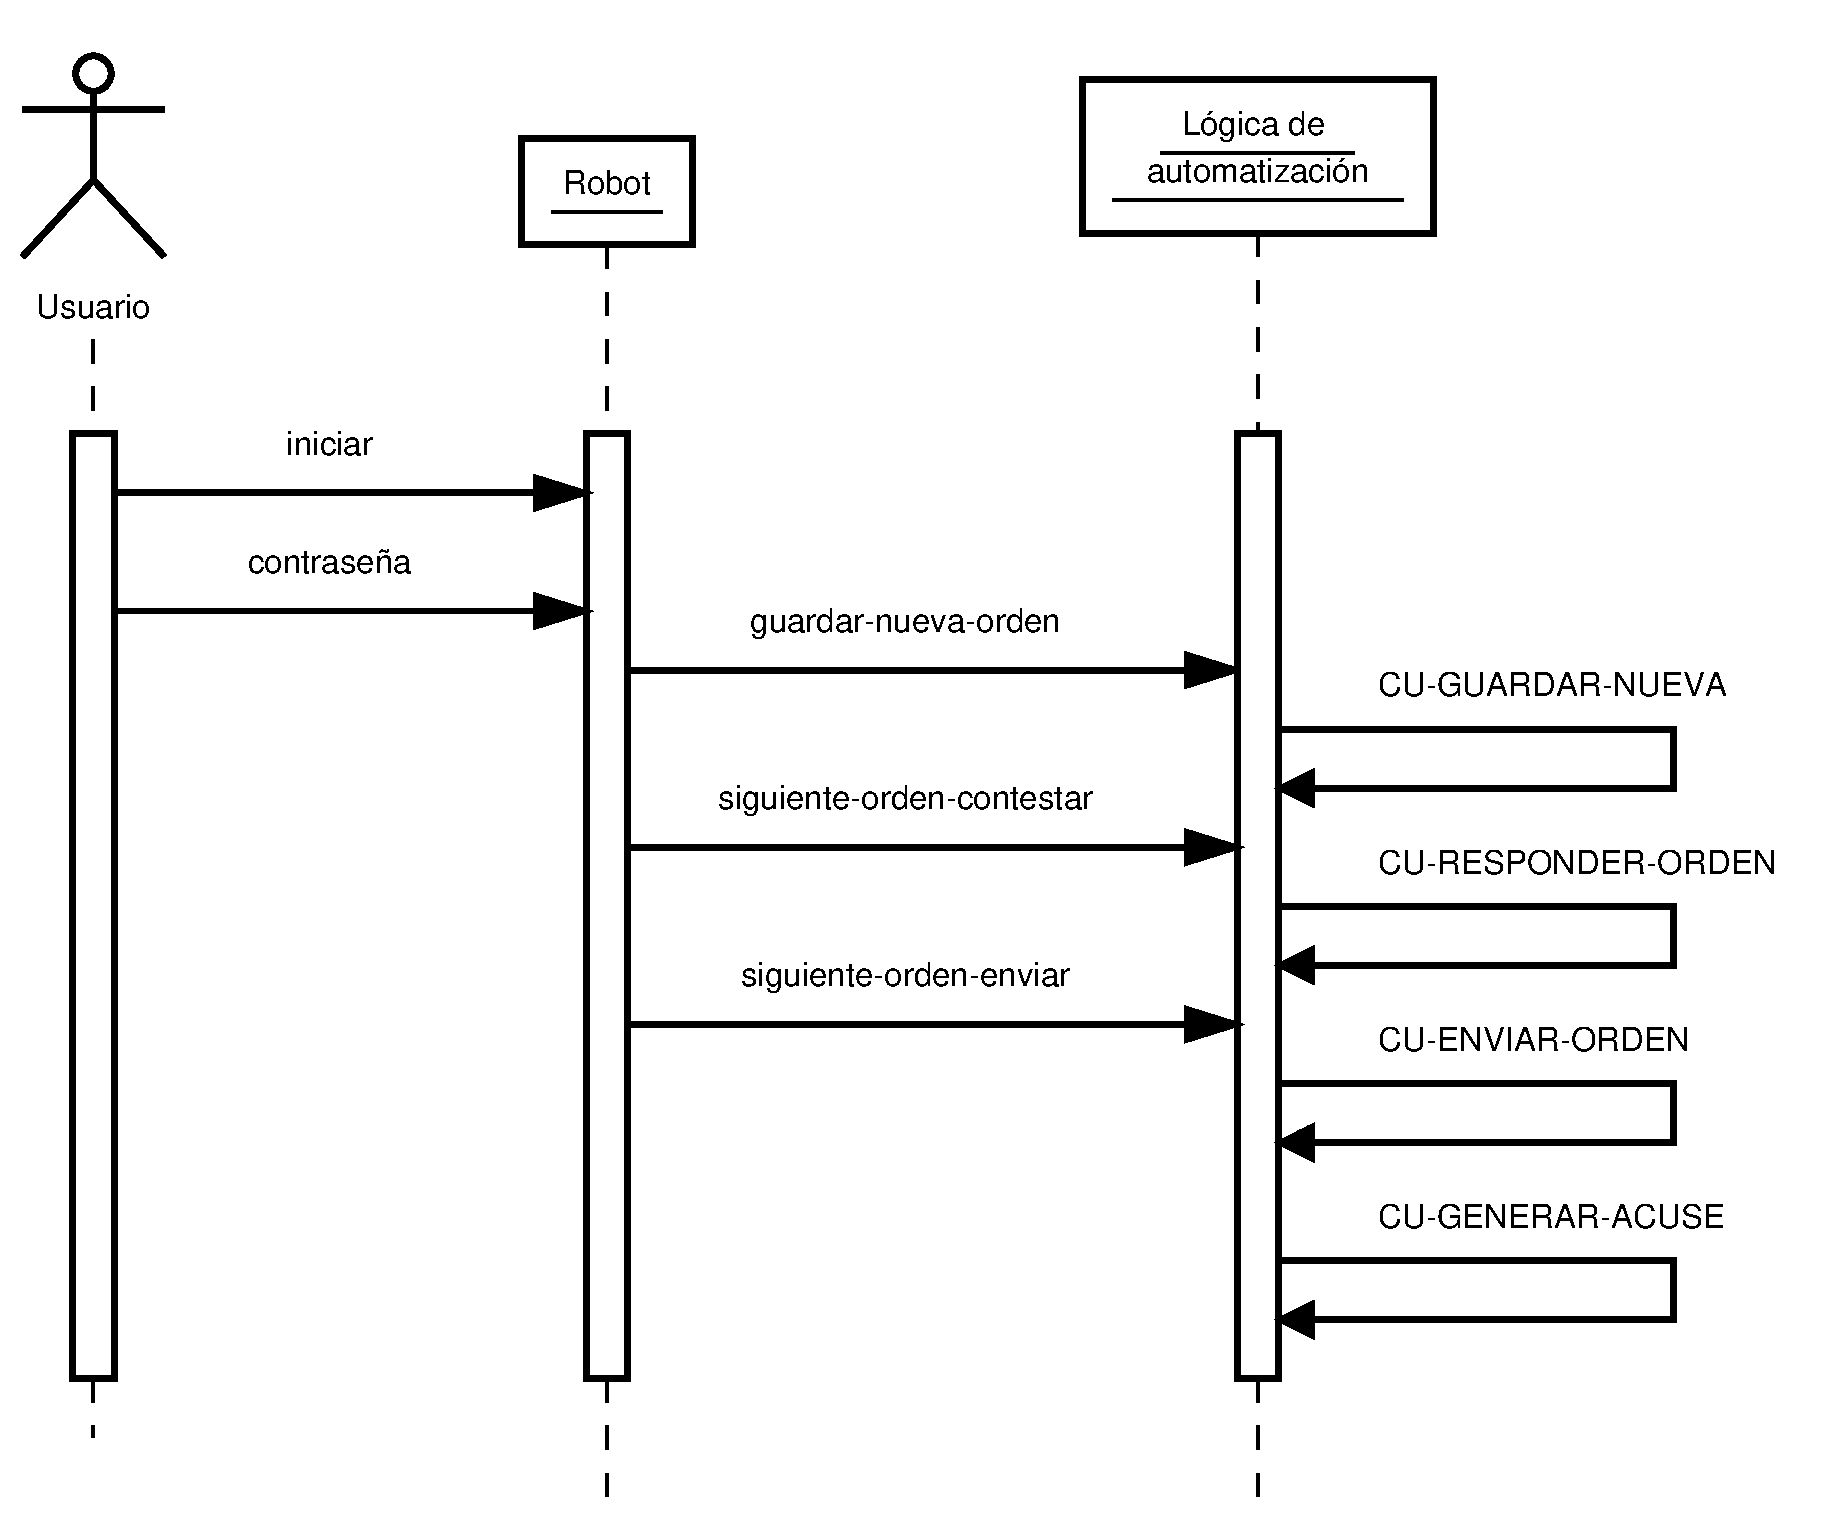
\includegraphics[scale=0.6]{dia-seq-cu-contestar}
	\caption{Diagrama de secuencia del caso de uso CU-CONTESTAR.}
	\label{fig:dia-seq-cu-contestar}
\end{figure}

\subsubsection{Guardar nueva orden}
El diseño para la solución del caso de uso \textbf{CU-GUARDAR-NUEVA} (sección \ref{cu-guardar-nueva}) utiliza los componentes \textbf{Agente}, \textbf{Lógica de Automatización} y \textbf{Persistencia}. Tal solución se logra realizando las siguientes llamadas (Figura \ref{fig:dia-seq-cu-guardar-nueva}):
\begin{enumerate}
	\item \textbf{Agente}: envía los datos de la nueva orden de reposición (mensaje 1 del diagrama de la Figura \ref{fig:dia-seq-cu-guardar-nueva}).
	\item \textbf{Lógica de Automatización}: de encontrarse, remueve los espacios en blanco al principio y al final de cada dato de la orden.
	\item \textbf{Lógica de Automatización}: construye la \textit{URL de envío} de la orden de reposición.
	\item \textbf{Lógica de Automatización}: envía la orden de reposición al componente de persistencia, (mensaje 2 del diagrama de la Figura \ref{fig:dia-seq-cu-guardar-nueva}).
	\item \textbf{Persistencia}: almacena la orden de reposición en la base de datos.
\end{enumerate}

\begin{figure}[h]
	\centering
	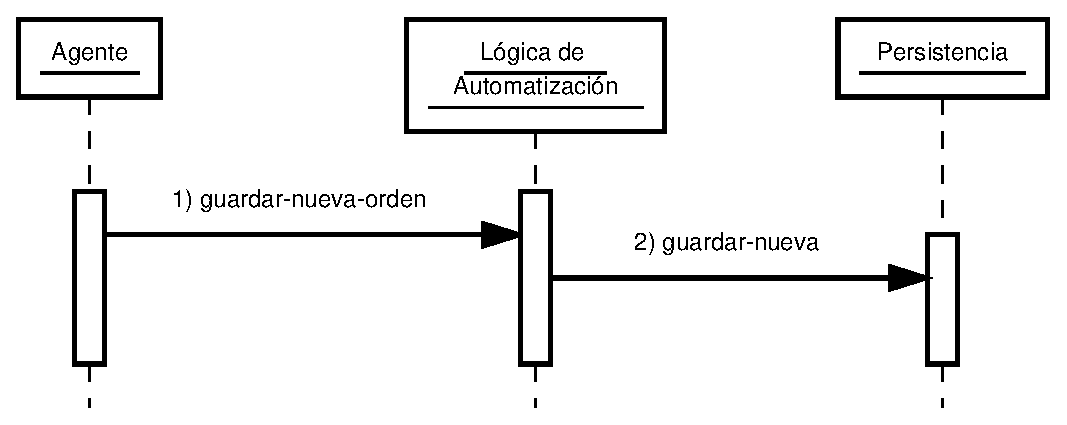
\includegraphics[scale=0.6]{dia-seq-cu-guardar-nueva}
	\caption{Diagrama de secuencia del caso de uso CU-GUARDAR-NUEVA.}
	\label{fig:dia-seq-cu-guardar-nueva}
\end{figure}

\subsubsection{Responder orden}
El diseño para la solución del caso de uso \textbf{CU-RESPONDER-ORDEN} (sección \ref{cu-responder-orden}) utiliza los componentes \textbf{Agente}, \textbf{Lógica de Automatización} y \textbf{Persistencia}. Tal solución se logra realizando las siguientes llamadas (Figura \ref{fig:dia-seq-cu-responder-orden}):
\begin{enumerate}
	\item \textbf{Agente}: solicita la siguiente orden de reposición para contestar (mensaje 1 del diagrama de la Figura \ref{fig:dia-seq-cu-responder-orden}).
	\item \textbf{Lógica de Automatización}: consulta el componente \textbf{Persistencia} para obtener la siguiente orden para contestar.
	\item \textbf{Persistencia}: obtiene la primera orden de reposición con estado de \textbf{Nueva}.
	\item \textbf{Persistencia}: cambia el estado de la orden a \textbf{Siendo Contestada} (mensaje 3 del diagrama de la Figura \ref{fig:dia-seq-cu-responder-orden}).
	\item \textbf{Agente}: solicita los datos para llenar los formularios (mensaje 6 del diagrama de la Figura \ref{fig:dia-seq-cu-responder-orden}).
	\item \textbf{Agente}: solicita almacenar los datos de la orden de reposición contestada (mensaje 7 del diagrama de la Figura \ref{fig:dia-seq-cu-responder-orden}).
	\item \textbf{Lógica de Automatización}: envía los datos de la orden contestada al componente \textbf{Persistencia} para que sean almacenados (mensaje 8 del diagrama de la Figura \ref{fig:dia-seq-cu-responder-orden}).
	\item \textbf{Lógica de Automatización}: manda el cambio de estado de la orden a \textbf{Contestada} (mensaje 9 del diagrama de la Figura \ref{fig:dia-seq-cu-responder-orden}).
\end{enumerate}

\begin{figure}[h]
	\centering
	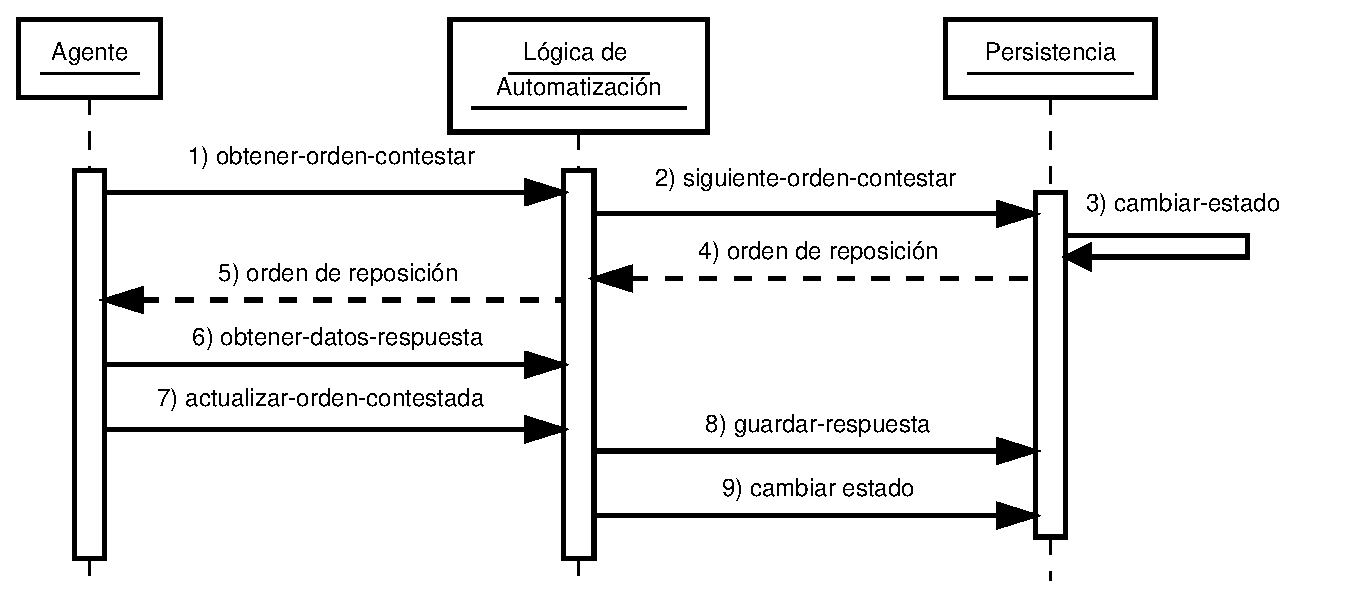
\includegraphics[scale=0.6]{dia-seq-cu-responder-orden}
	\caption{Diagrama de secuencia del caso de uso CU-RESPONDER-ORDEN.}
	\label{fig:dia-seq-cu-responder-orden}
\end{figure}

\subsubsection{Enviar orden}
El diseño para la solución del caso de uso \textbf{CU-ENVIAR-ORDEN} (sección \ref{cu-enviar-orden}) utiliza los componentes \textbf{Agente}, \textbf{Lógica de Automatización} y \textbf{Persistencia}. Tal solución se logra realizando las siguientes llamadas (Figura \ref{fig:dia-seq-cu-enviar-orden}):
\begin{enumerate}
	\item \textbf{Agente}: solicita la siguiente orden de reposición para enviar (mensaje 1 del diagrama de la Figura \ref{fig:dia-seq-cu-enviar-orden}).
	\item \textbf{Lógica de Automatización}: consulta el componente \textbf{Persistencia} para obtener la siguiente orden para enviar (mensaje 2 del diagrama de la Figura \ref{fig:dia-seq-cu-enviar-orden}).
	\item \textbf{Persistencia}: obtiene la primera orden de reposición con estado de \textbf{Contestada}.
	\item \textbf{Persistencia}: cambia el estado de la orden a \textbf{Siendo Enviada} (mensaje 3 del diagrama de la Figura \ref{fig:dia-seq-cu-enviar-orden}).
	\item \textbf{Agente}: dirige el explorador de internet a la \textit{URL de envío}.
	\item \textbf{Agente}: manda almacenar el folio de envío (mensaje 6 del diagrama de la Figura \ref{fig:dia-seq-cu-enviar-orden}).
	\item \textbf{Lógica de Automatización}: utiliza el componente \textbf{Persistencia} para almacenar el folio de envío (mensaje 7 del diagrama de la Figura \ref{fig:dia-seq-cu-enviar-orden}).
	\item \textbf{Lógica de Automatización}: actualiza el estado de la orden a \textbf{Enviada} (mensaje 8 del diagrama de la Figura \ref{fig:dia-seq-cu-enviar-orden}).
\end{enumerate}

\begin{figure}[h]
	\centering
	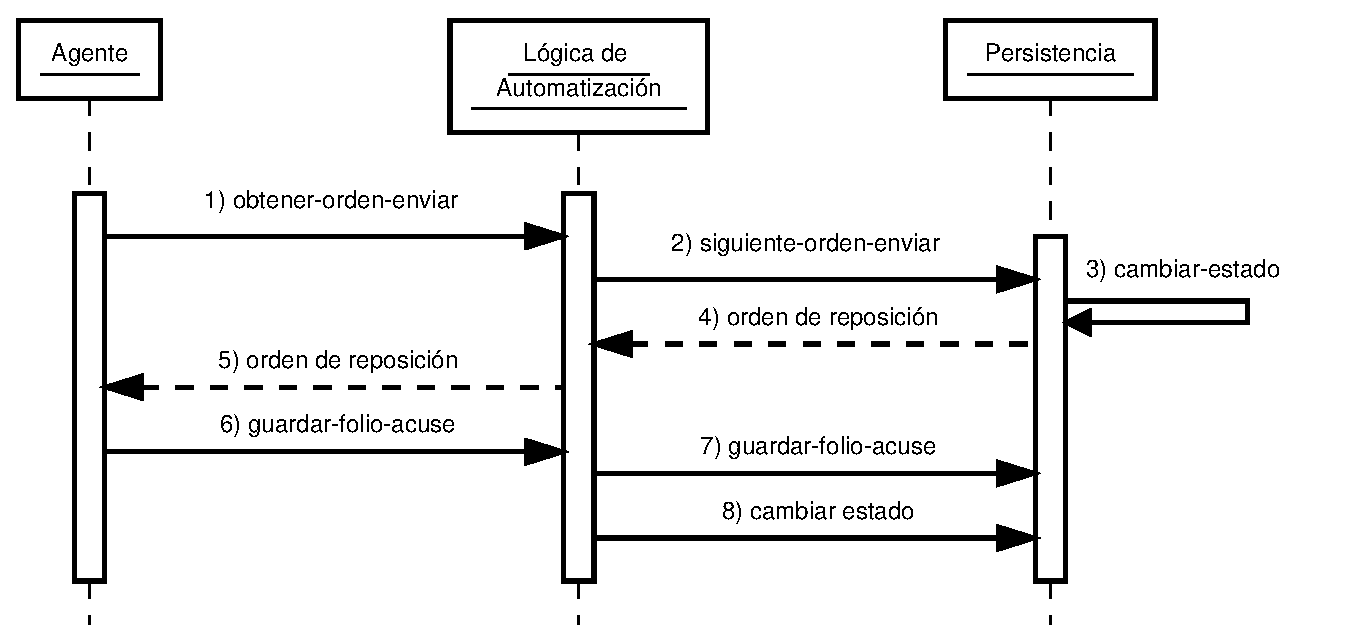
\includegraphics[scale=0.6]{dia-seq-cu-enviar-orden}
	\caption{Diagrama de secuencia del caso de uso CU-ENVIAR-ORDEN.}
	\label{fig:dia-seq-cu-enviar-orden}
\end{figure}

\subsubsection{Generar acuse de envío}
El diseño para la solución del caso de uso \textbf{CU-GENERAR-ACUSE} (sección \ref{cu-generar-acuse}) utiliza los componentes \textbf{Lógica de Automatización}, \textbf{Persistencia}, \textbf{Generador de Reportes} y \textbf{Ficheros}. Tal solución se logra realizando las siguientes llamadas (Figura \ref{fig:dia-seq-cu-generar-acuse}):
\begin{enumerate}
	\item \textbf{Lógica de Automatización}: solicita los datos de la orden de reposición al componente \textbf{Persistencia} (mensaje 1 del diagrama de la Figura \ref{fig:dia-seq-cu-generar-acuse}).
	\item \textbf{Lógica de Automatización}: solicita la generación del acuse de envío al componente \textbf{Generador de Reportes} (mensaje 2 del diagrama de la Figura \ref{fig:dia-seq-cu-generar-acuse}).
	\item \textbf{Generador de Reportes}: solicita almacenar el acuse de envío al componente \textbf{Ficheros} (mensaje 3 del diagrama de la Figura \ref{fig:dia-seq-cu-generar-acuse}).
\end{enumerate}

\begin{figure}[h]
	\centering
	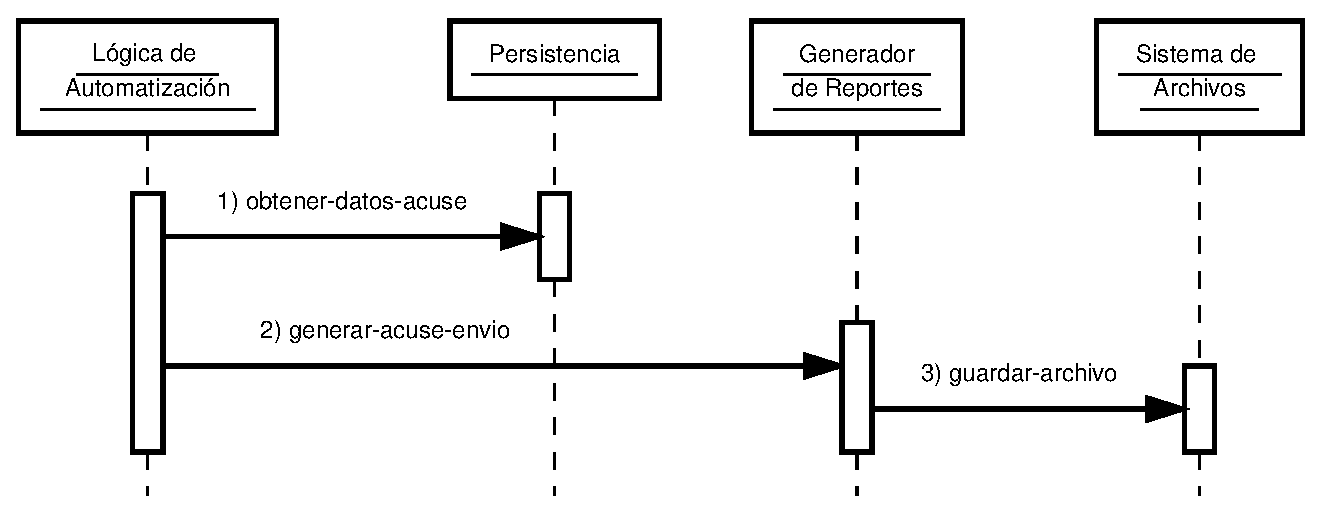
\includegraphics[scale=0.6]{dia-seq-cu-generar-acuse}
	\caption{Diagrama de secuencia del caso de uso CU-GENERAR-ACUSE.}
	\label{fig:dia-seq-cu-generar-acuse}
\end{figure}

%espaciado
\pagebreak
%espaciado

\subsubsection{Verificar órdenes}
El diseño de la solución al caso de uso \textbf{CU-VERIFICAR} (sección \ref{cu-verificar}) se lleva a cabo entre el actor \textbf{Usuario} y los componentes \textbf{Agente} \textbf{Lógica de Automatización}. Tal solución se logra realizando las siguientes llamadas (Figura \ref{fig:dia-seq-cu-verificar}):
\begin{enumerate}
	\item \textbf{Usuario}: inicia la ejecución del agente (mensaje 1 del diagrama de la Figura \ref{fig:dia-seq-cu-verificar}).
	\item \textbf{Agente}: dirige el explorador de internet a la página del \textit{Sistema de Abastecimiento} y solicita al usuario la contraseña para ingresar.
	\item \textbf{Usuario}: proporciona la contraseña (mensaje 2 del diagrama de la Figura \ref{fig:dia-seq-cu-verificar}).
	\item \textbf{Agente}: realiza el acceso al \textit{Sistema de Abastecimiento}.
	\item \textbf{Agente}: dirige el explorador de internet a la búsqueda de órdenes de reposición.
	\item \textbf{Agente}: solicita el rango de fechas al componente \textbf{Lógica de Automatización} (mensaje 3 del diagrama de la Figura \ref{fig:dia-seq-cu-verificar}).
	\item \textbf{Agente}: realiza la búsqueda de órdenes de reposición canceladas.
	\item \textbf{Agente}: envía el listado con los números de orden de reposición resultantes al componente \textbf{Lógica de Automatización} (mensaje 4 del diagrama de la Figura \ref{fig:dia-seq-cu-verificar}).
	\item \textbf{Lógica de Automatización}: ejecuta los casos de uso \textbf{CU-ACTUALIZAR-ESTATUS-SA} (mensaje 5 del diagrama de la Figura \ref{fig:dia-seq-cu-verificar}).
\end{enumerate}

\begin{figure}[h]
	\centering
	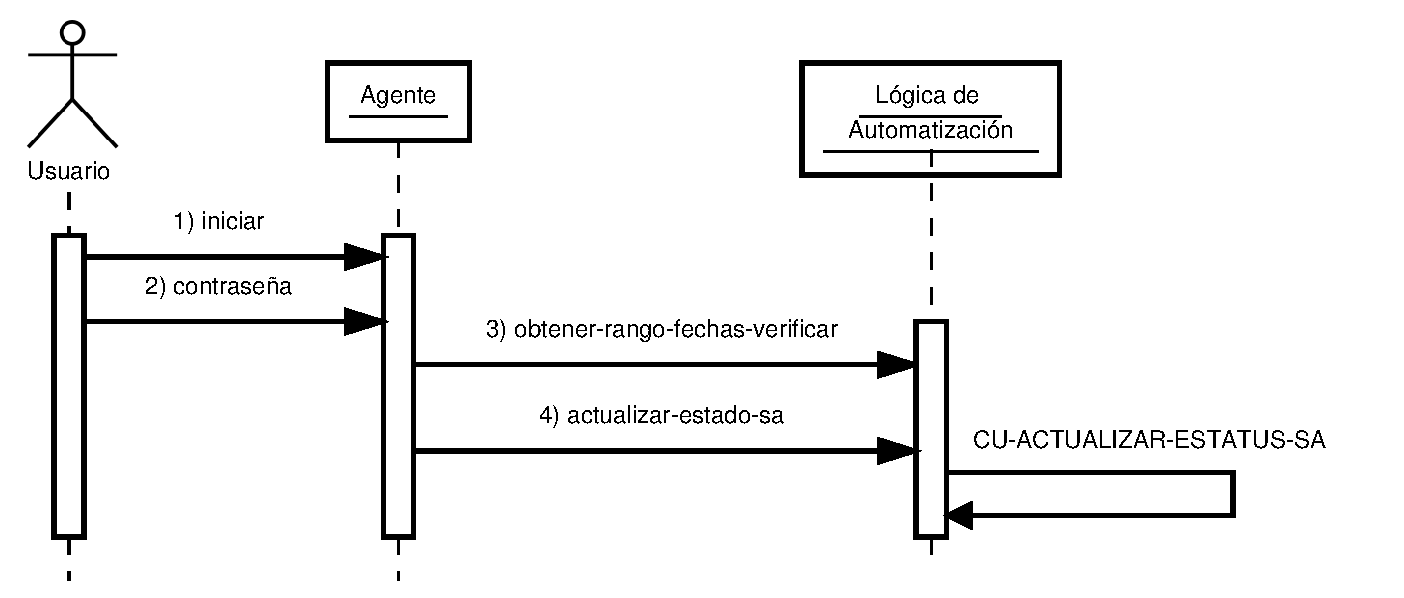
\includegraphics[scale=0.6]{dia-seq-cu-verificar}
	\caption{Diagrama de secuencia del caso de uso CU-VERIFICAR.}
	\label{fig:dia-seq-cu-verificar}
\end{figure}

\subsubsection{Actualizar estatus de Sistema de Abastecimiento}
El diseño para la solución del caso de uso \textbf{CU-ACTUALIZAR-ESTATUS-SA} (sección \ref{cu-actualizar-estatus-sa}) utiliza los componentes \textbf{Agente}, \textbf{Lógica de Automatización} y \textbf{Persistencia}. Tal solución se logra realizando las siguientes llamadas (Figura \ref{fig:dia-seq-cu-actualizar-estatus-sa}):
\begin{enumerate}
	\item \textbf{Lógica de Automatización}: envía el listado de con los números de órdenes de reposición al componente \textbf{Persistencia} para actualizar en la base de datos el estado conocido en el \textit{Sistema de Abastecimiento} (mensaje 1 del diagrama de la Figura \ref{fig:dia-seq-cu-actualizar-estatus-sa}).
\end{enumerate}

\begin{figure}[h]
	\centering
	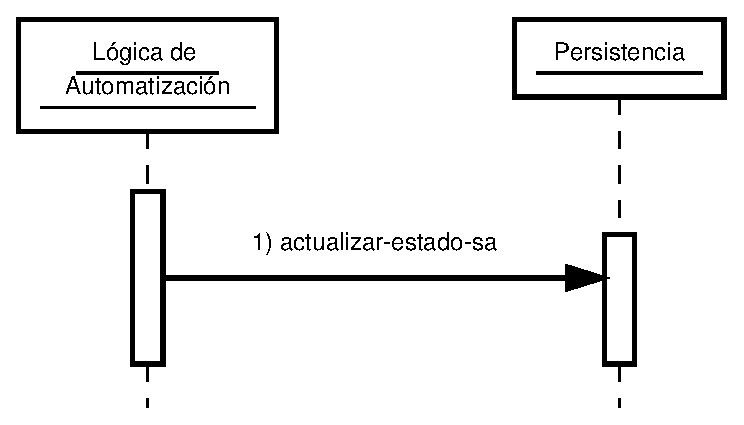
\includegraphics[scale=0.6]{dia-seq-cu-actualizar-estatus-sa}
	\caption{Diagrama de secuencia del caso de uso CU-ACTUALIZAR-ESTATUS-SA.}
	\label{fig:dia-seq-cu-actualizar-estatus-sa}
\end{figure}

%espaciado
\pagebreak
%espaciado
\subsubsection{Entrar en interfaz web}
El diseño de la solución al caso de uso \textbf{CU-ENTRAR-WEB} (sección \ref{cu-entrar-web}) se lleva a cabo entre el actor \textbf{Usuario} y los componentes \textbf{Portal Web} y \textbf{Persistencia}. Tal solución se logra realizando las siguientes llamadas (Figura \ref{fig:dia-seq-cu-entrar-web}):
\begin{enumerate}
	\item \textbf{Usuario}: introduce su nombre de usuario y contraseña, tal pareja es referida como \textbf{credenciales} (mensaje 1 del diagrama de la Figura \ref{fig:dia-seq-cu-entrar-web}).
	\item \textbf{Portal Web}: envía el nombre de usuario al componente \textbf{Persistencia} que realiza la búsqueda de los datos del usuario (mensaje 2 del diagrama de la Figura \ref{fig:dia-seq-cu-entrar-web}).
	\item \textbf{Portal Web}: compara la contraseña con la almacenada en la base de datos.
	\begin{enumerate}
		\item Si las credenciales son válidas: el \textbf{Portal Web} regresa al \textbf{Usuario} un código de acceso temporal (mensaje 3 del diagrama de la Figura \ref{fig:dia-seq-cu-entrar-web}).
		\item Si las credenciales son inválidas: el \textbf{Portal Web} regresa al \textbf{Usuario} un mensaje de error (mensaje 4 del diagrama de la Figura \ref{fig:dia-seq-cu-entrar-web}).
	\end{enumerate}
\end{enumerate}

\begin{figure}[h]
	\centering
	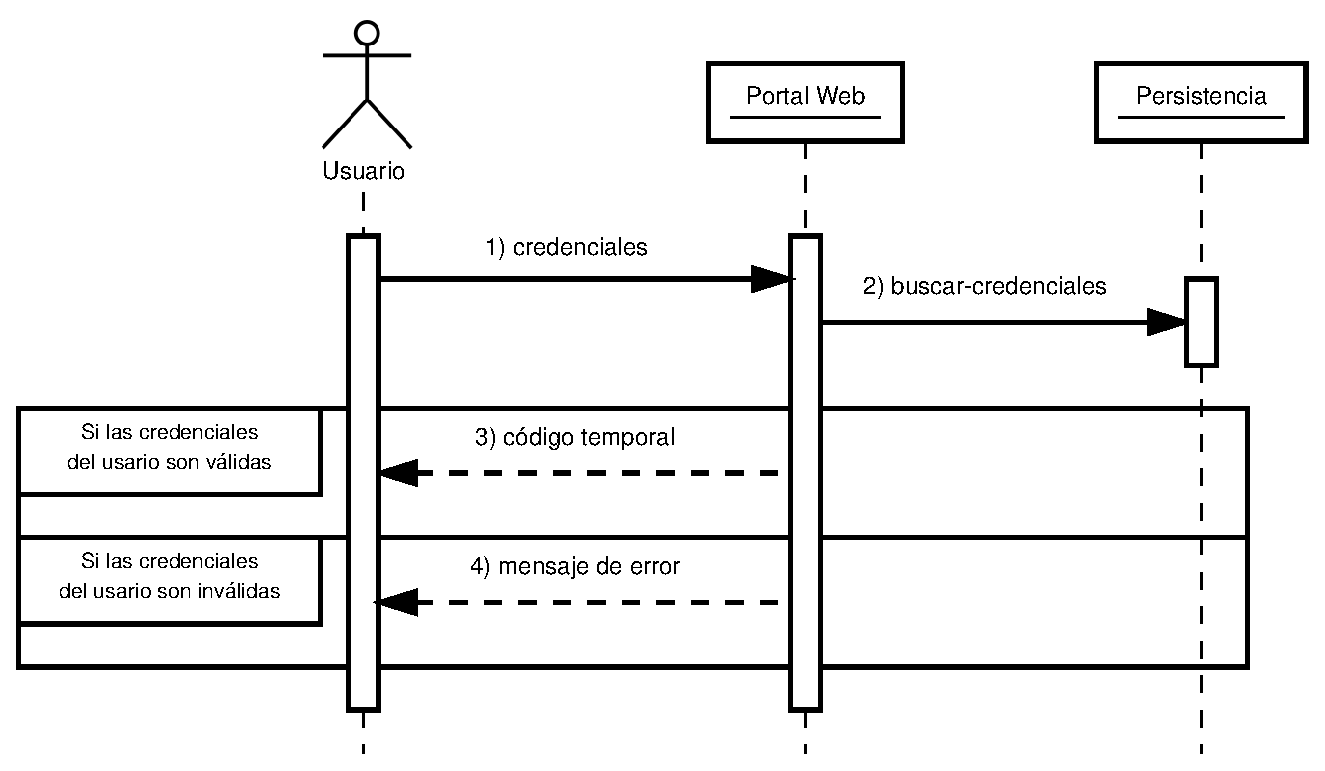
\includegraphics[scale=0.6]{dia-seq-cu-entrar-web}
	\caption{Diagrama de secuencia del caso de uso CU-ENTRAR-WEB.}
	\label{fig:dia-seq-cu-entrar-web}
\end{figure}

\subsubsection{Generar reporte}
El diseño de la solución al caso de uso \textbf{CU-GENERAR-REPORTE} (sección \ref{cu-generar-reporte}) se lleva a cabo entre el actor \textbf{Usuario} y los componentes \textbf{Portal Web}, \textbf{Persistencia}, \textbf{Generador de Reportes} y \textbf{Ficheros}. Tal solución se logra realizando las siguientes llamadas (Figura \ref{fig:dia-seq-cu-generar-reporte}):
\begin{enumerate}
	\item \textbf{Usuario}: selecciona el tipo de reporte y el rango de fechas (mensaje 1 del diagrama de la Figura \ref{fig:dia-seq-cu-generar-reporte}).
	\item \textbf{Portal Web}: solicita la búsqueda de órdenes al componente \textbf{Persistencia} (mensaje 2 del diagrama de la Figura \ref{fig:dia-seq-cu-generar-reporte}).
	\item \textbf{Portal Web}: envía las órdenes para generar el reporte (mensaje 3 del diagrama de la Figura \ref{fig:dia-seq-cu-generar-reporte}).
	\item \textbf{Generador de Reportes}: genera el reporte.
	\item \textbf{Generador de Reportes}: solicita al componente \textbf{Ficheros} almacenar el reporte (mensaje 4 del diagrama de la Figura \ref{fig:dia-seq-cu-generar-reporte}).
	\item \textbf{Generador de Reportes}: regresa la ruta donde se guardó el reporte (mensaje 5 del diagrama de la Figura \ref{fig:dia-seq-cu-generar-reporte}).
	\item \textbf{Portal Web}: muestra al \textbf{Usuario} la ruta donde se encuentra el reporte (mensaje 6 del diagrama de la Figura \ref{fig:dia-seq-cu-generar-reporte}).
\end{enumerate}

\begin{figure}[h]
	\centering
	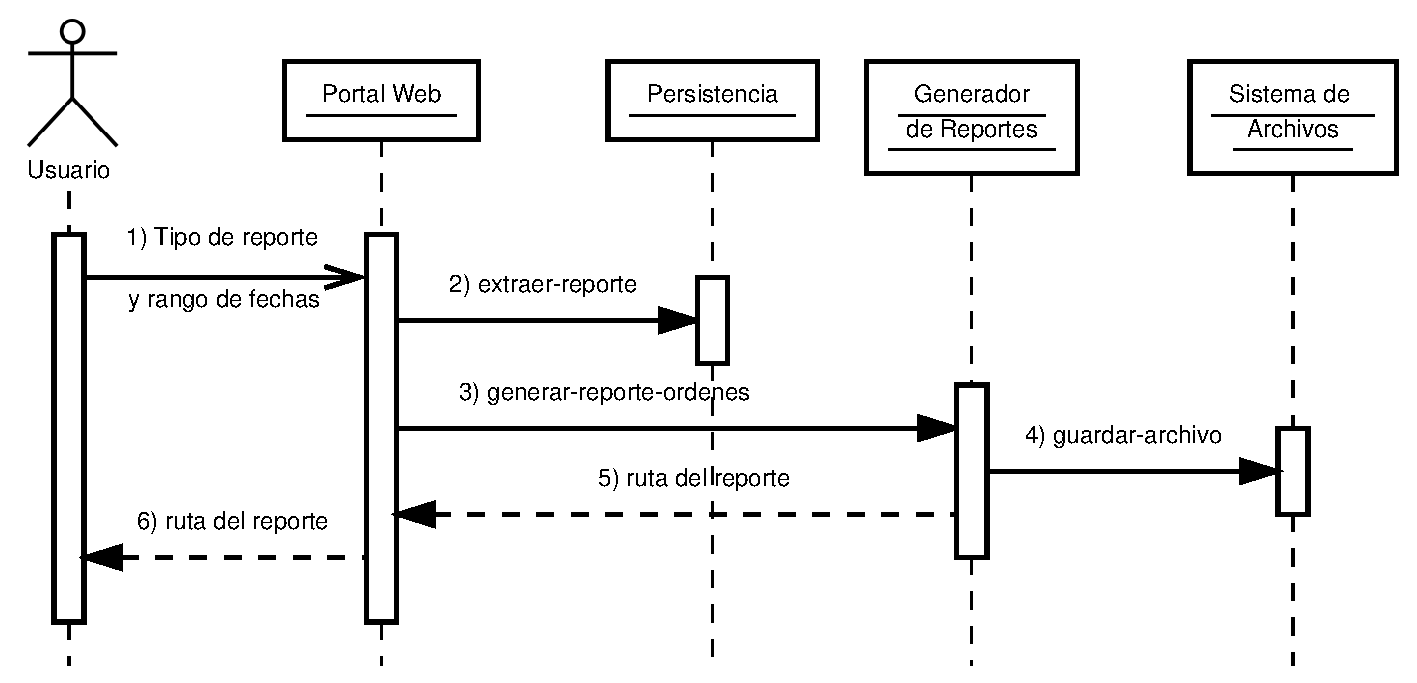
\includegraphics[scale=0.6]{dia-seq-cu-generar-reporte}
	\caption{Diagrama de secuencia del caso de uso CU-GENERAR-REPORTE.}
	\label{fig:dia-seq-cu-generar-reporte}
\end{figure}

%espaciado
\pagebreak
%espaciado

\subsubsection{Actualizar catálogo}
El diseño de la solución al caso de uso \textbf{CU-ACTUALIZAR-CATALOGO} (sección \ref{cu-actualizar-catalogo}) se lleva a cabo entre el actor \textbf{Usuario} y los componentes \textbf{Portal Web} y \textbf{Persistencia}. Tal solución se logra realizando las siguientes llamadas (Figura \ref{fig:dia-seq-cu-actualizar-catalogo}):
\begin{enumerate}
	\item \textbf{Usuario}: selecciona el catálogo y el archivo (mensaje 1 del diagrama de la Figura \ref{fig:dia-seq-cu-actualizar-catalogo}).
	\item \textbf{Portal Web}: solicita la actualización del catálogo al componente \textbf{Persistencia} (mensaje 2 del diagrama de la Figura \ref{fig:dia-seq-cu-actualizar-catalogo}).
	\item \textbf{Portal Web}: muestra al \textbf{Usuario} la cantidad de registros almacenados (mensaje 3 del diagrama de la Figura \ref{fig:dia-seq-cu-actualizar-catalogo}).
\end{enumerate}

\begin{figure}[h]
	\centering
	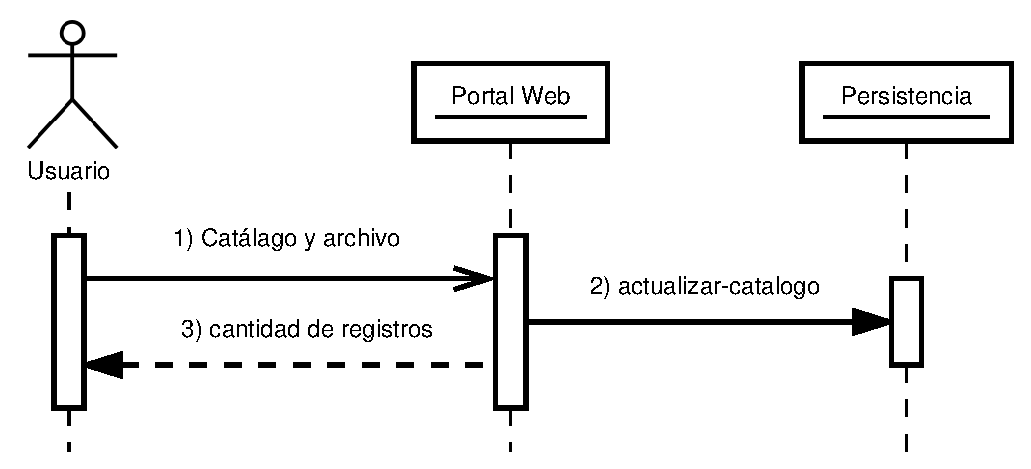
\includegraphics[scale=0.6]{dia-seq-cu-actualizar-catalogo}
	\caption{Diagrama de secuencia del caso de uso CU-ACTUALIZAR-CATALOGO.}
	\label{fig:dia-seq-cu-actualizar-catalogo}
\end{figure}

%espaciado
\pagebreak
%espaciado

\subsubsection{Buscar órdenes}
El diseño de la solución al caso de uso \textbf{CU-BUSCAR} (sección \ref{cu-buscar}) se lleva a cabo entre el actor \textbf{Usuario} y los componentes \textbf{Portal Web} y \textbf{Persistencia}. Tal solución se logra realizando las siguientes llamadas (Figura \ref{fig:dia-seq-cu-buscar}):
\begin{enumerate}
	\item \textbf{Usuario}: llena el formulario de búsqueda \textbf{filtro} (mensaje 1 del diagrama de la Figura \ref{fig:dia-seq-cu-buscar}).
	\item \textbf{Portal Web}: solicita la realización de la búsqueda de órdenes al componente \textbf{Persistencia} (mensaje 2 del diagrama de la Figura \ref{fig:dia-seq-cu-buscar}).
	\item \textbf{Portal Web}: muestra al \textbf{Usuario} el listado de órdenes de reposición encontradas (mensaje 3 del diagrama de la Figura \ref{fig:dia-seq-cu-buscar}).
\end{enumerate}

\begin{figure}[h]
	\centering
	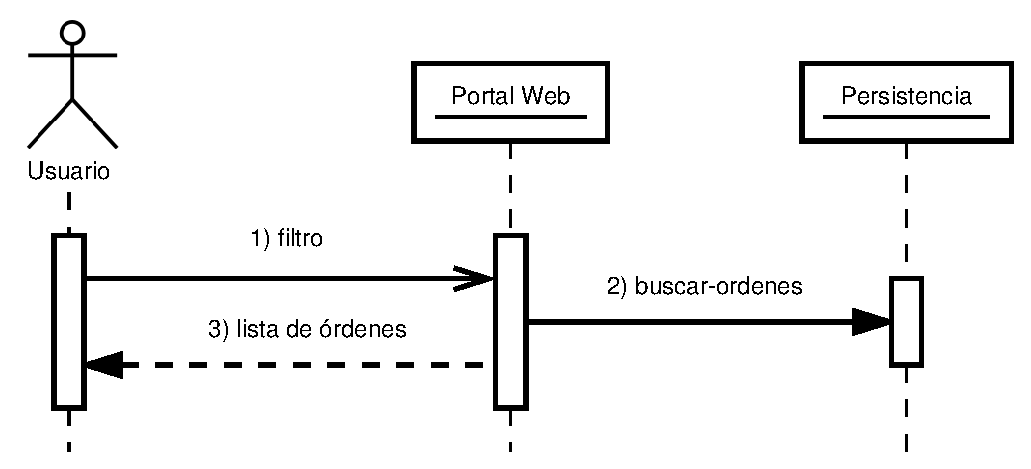
\includegraphics[scale=0.6]{dia-seq-cu-buscar}
	\caption{Diagrama de secuencia del caso de uso CU-BUSCAR.}
	\label{fig:dia-seq-cu-buscar}
\end{figure}

\subsubsection{Visualizar orden}
El diseño de la solución al caso de uso \textbf{CU-VISUALIZAR} (sección \ref{cu-visualizar}) se lleva a cabo entre el actor \textbf{Usuario} y los componentes \textbf{Portal Web} y \textbf{Persistencia}. Tal solución se logra realizando las siguientes llamadas (Figura \ref{fig:dia-seq-cu-visualizar}):
\begin{enumerate}
	\item \textbf{Usuario}: selecciona la orden de reposición (mensaje 1 del diagrama de la Figura \ref{fig:dia-seq-cu-visualizar}).
	\item \textbf{Portal Web}: solicita la realización de la búsqueda de la orden al componente \textbf{Persistencia} (mensaje 2 del diagrama de la Figura \ref{fig:dia-seq-cu-visualizar}).
	\item \textbf{Portal Web}: muestra al \textbf{Usuario} la información de la orden de reposición.
\end{enumerate}

\begin{figure}[h]
	\centering
	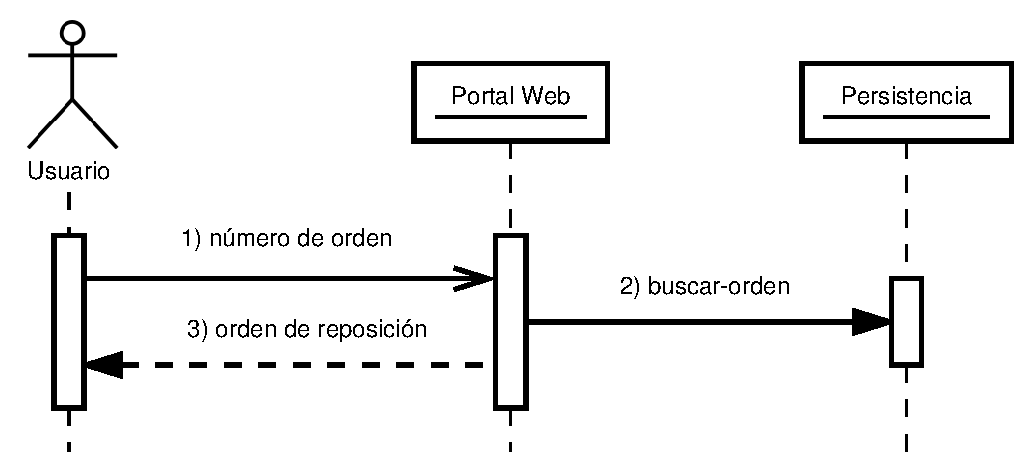
\includegraphics[scale=0.6]{dia-seq-cu-visualizar}
	\caption{Diagrama de secuencia del caso de uso CU-VISUALIZAR.}
	\label{fig:dia-seq-cu-visualizar}
\end{figure}

\subsubsection{Editar orden}
El diseño de la solución al caso de uso \textbf{CU-EDITAR} (sección \ref{cu-editar}) se lleva a cabo entre el actor \textbf{Usuario} y los componentes \textbf{Portal Web} y \textbf{Persistencia}. Tal solución se logra realizando las siguientes llamadas (Figura \ref{fig:dia-seq-cu-editar}):
\begin{enumerate}
	\item \textbf{Usuario}: activa la edición de la orden de reposición (mensaje 1 del diagrama de la Figura \ref{fig:dia-seq-cu-editar}).
	\item \textbf{Usuario}: modifica la información de la orden de reposición (mensaje 2 de la Figura \ref{fig:dia-seq-cu-editar}).
	\item \textbf{Portal Web}: solicita la actualización de la orden al componente \textbf{Persistencia} (mensaje 3 del diagrama de la Figura \ref{fig:dia-seq-cu-editar}).
\end{enumerate}

\begin{figure}[h]
	\centering
	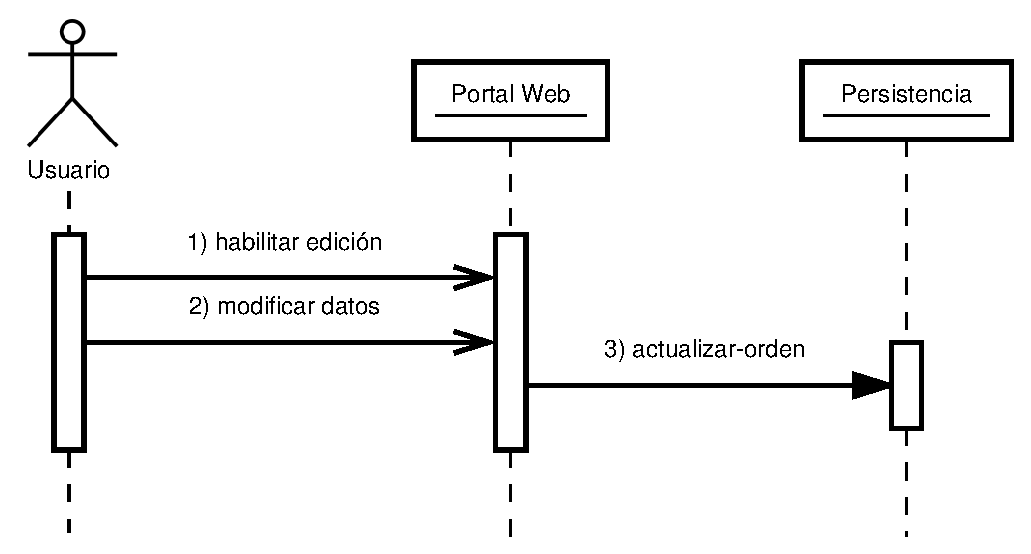
\includegraphics[scale=0.6]{dia-seq-cu-editar}
	\caption{Diagrama de secuencia del caso de uso CU-EDITAR.}
	\label{fig:dia-seq-cu-editar}
\end{figure}


%===============================================================================
%===============================================================================

\section{Diseño de la base de datos}
La base de datos tiene dos finalidades: la primera es guardar la información capturada de las órdenes de reposición atendidas, así como los catálogos necesarios para los procesos automatizados y la generación de reportes; la segunda es almacenar la información de los usuarios autorizados para utilizar el portal web.\\
El diseño de la base de datos se centra en los siguientes grupos (Figura \ref{fig:dia-er-resumen}\footnote{Los nombres de las tablas están escritos utilizando letras minúsculas de alfabeto inglés y guion bajo $([a-z]{\_})^+$.}):
\begin{enumerate}
	\item Tablas de las órdenes de reposición.
	\item Tablas del registro de eventos.
	\item Tablas de los usuarios de la interfaz web.
	\item Catálogos para generación de reportes.
\end{enumerate}
\begin{figure}[h]
  \centering
  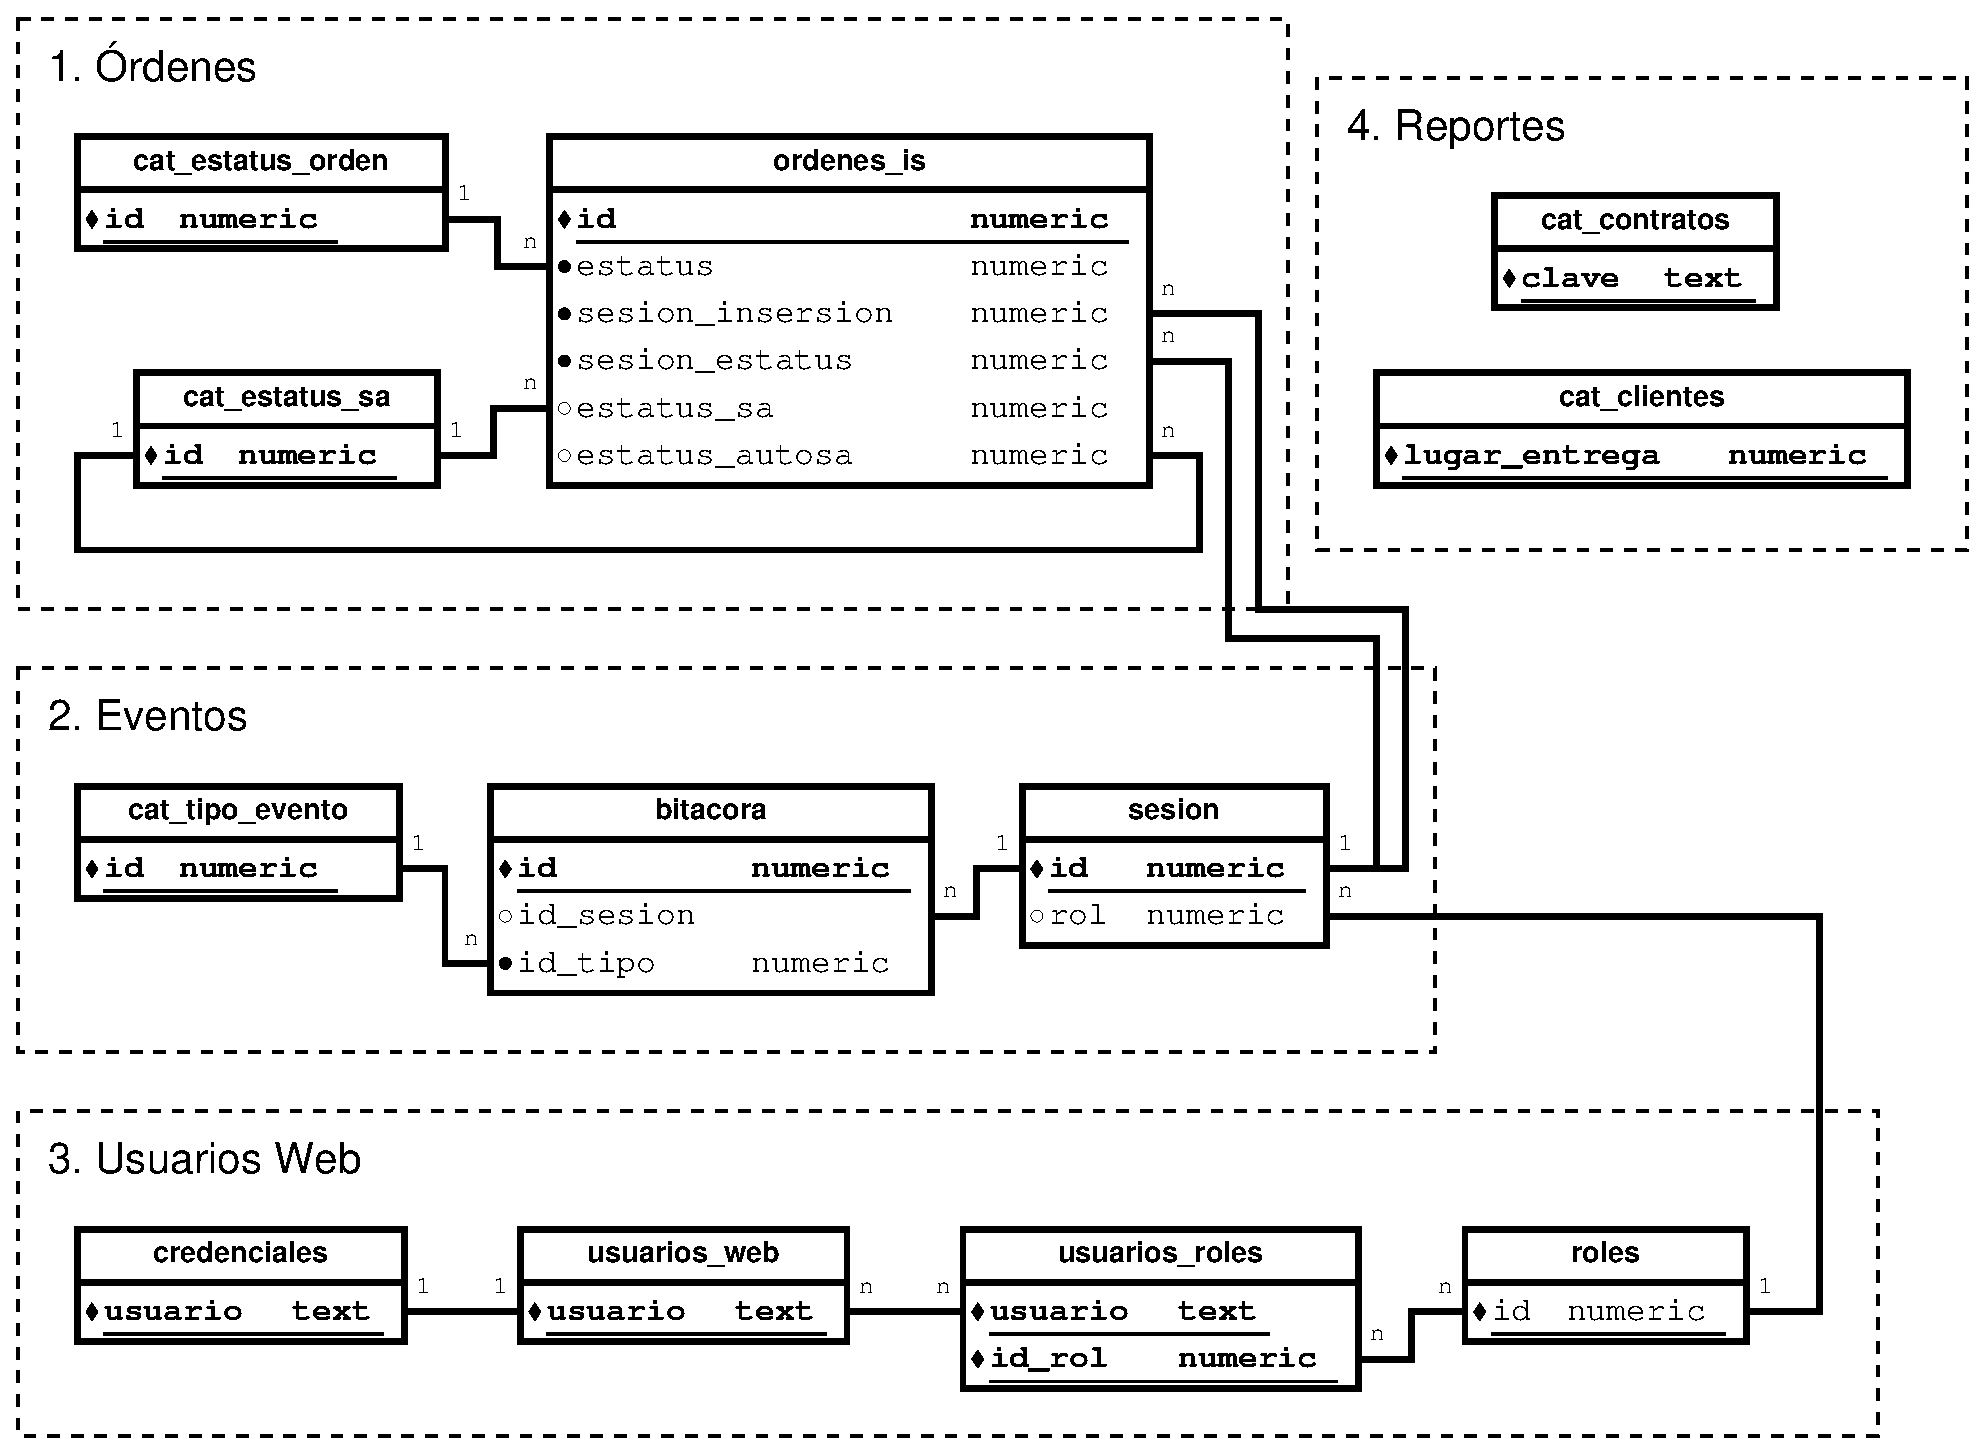
\includegraphics[width=\textwidth]{dia-er-resumen}
  \caption{Diagrama Entidad Relación de el Sistema AutoSA.}
  \label{fig:dia-er-resumen}
\end{figure}

% espaciado
\pagebreak
% espaciado

\subsection{Tablas de las órdenes de reposición}
En estas tablas (Figura \ref{fig:dia-er-ordenes}) se almacenan las órdenes de reposición atendidas durante la rutina automatizada para responder órdenes de reposición en el \textit{Sistema de Abastecimiento} (caso de uso \textbf{CU-CONTESTAR}). De igual manera, también son utilizadas en la verificación de órdenes de reposición canceladas (caso de uso \textbf{CU-VERIFICAR}).
\begin{figure}[h]
  \centering
  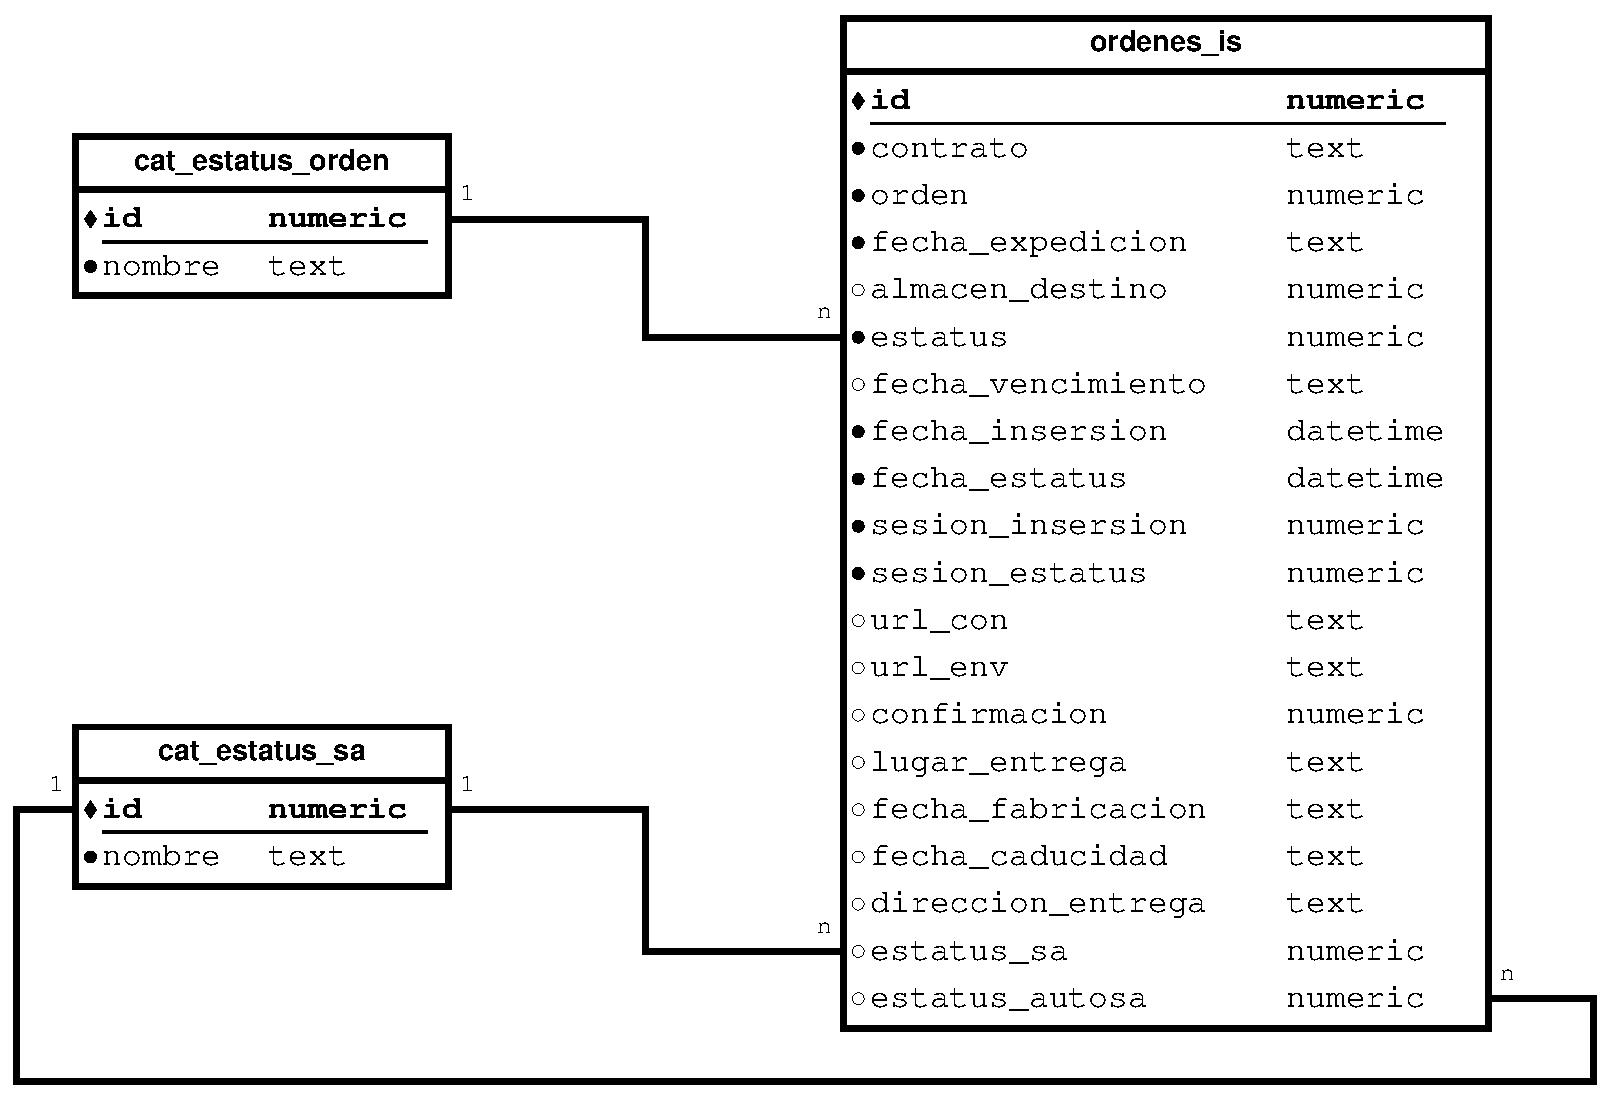
\includegraphics[scale=0.5]{dia-er-ordenes} 
  \caption{Diagrama Entidad Relación para el registro de órdenes de reposición.}
  \label{fig:dia-er-ordenes}
\end{figure}
\paragraph{ordenes{\textunderscore}is:} contiene el registro de las órdenes de reposición del \textit{Sistema de Abastecimiento} que han sido atendidas por la rutina de automatización.
\paragraph{cat{\textunderscore}estatus{\textunderscore}orden:} este catálogo no debe ser alterado. Contiene los posibles estados que puede tomar una orden durante el ciclo de vida de la aplicación.
\paragraph{cat{\textunderscore}estatus{\textunderscore}sa:} este catálogo contiene los estados definidos por el \textit{Sistema de Abastecimiento} para registrar y almacenar una orden de reposición.


\subsection{Tablas del registro de eventos}
El registro de eventos es todo lo relacionado con la actividad de los actores del sistema (agentes de automatización y usuarios), como se muestra en la Figura \ref{fig:dia-er-bitacora}.
\begin{figure}[h]
  \centering
  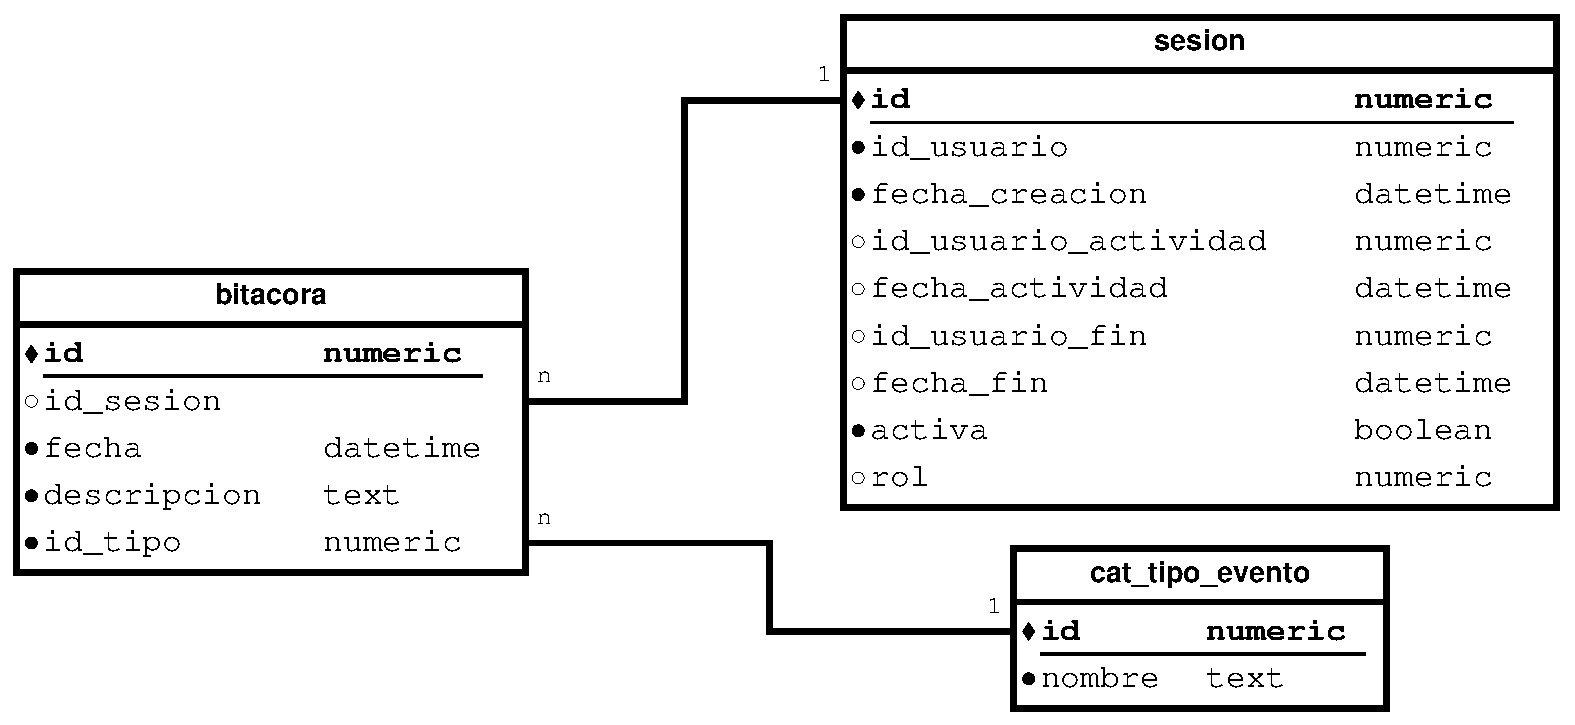
\includegraphics[scale=0.5]{dia-er-bitacora} 
  \caption{Diagrama Entidad Relación para el registro de eventos.}
  \label{fig:dia-er-bitacora}
\end{figure}
\paragraph{bitacora:} lleva el registro de eventos ocurridos durante la ejecución de las rutinas de automatización. El evento puede estar ligado a una sesión.
\paragraph{cat{\textunderscore}tipo{\textunderscore}evento:} se refiere al catálogo con los tipos de eventos que pueden ser registrados en la bitácora.
\paragraph{sesion:} define una sesión bajo la cual se ejecuta una rutina de automatización. La sesión puede definir implícitamente un usuario y un rol.


\subsection{Tablas de los usuarios de la interfaz web}
Las tablas de este grupo son utilizadas para gestionar el acceso a la interfaz web (caso de uso \textbf{CU-ENTRAR-WEB} y Figura \ref{fig:dia-er-web}).
\begin{figure}[h]
  \centering
  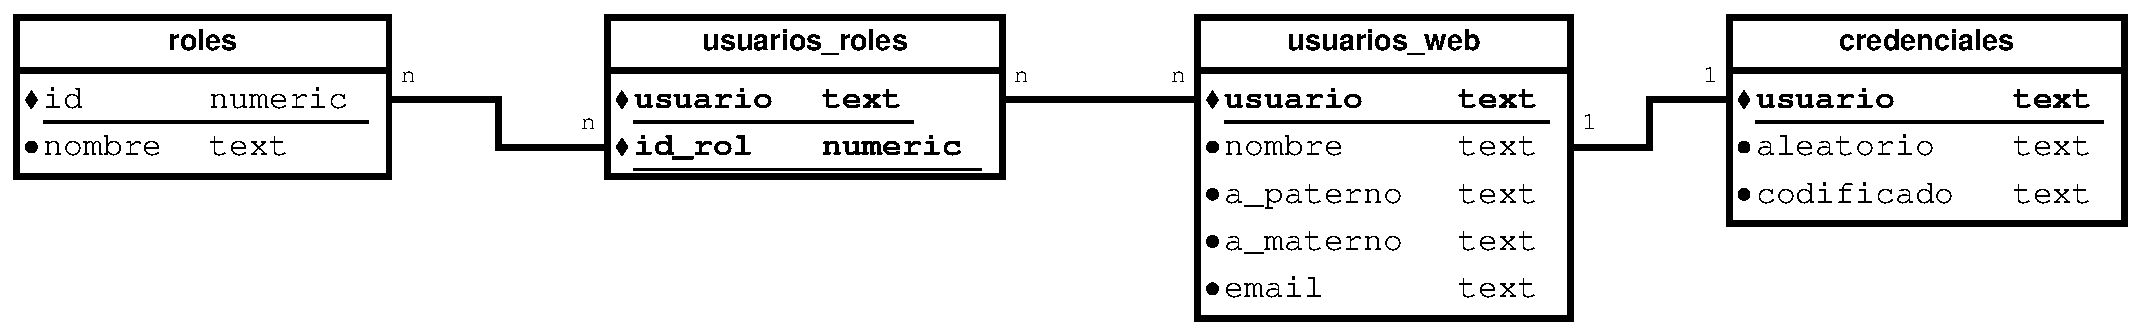
\includegraphics[scale=0.5]{dia-er-web} 
  \caption{Diagrama Entidad Relación para el manejo de usuarios.}
  \label{fig:dia-er-web}
\end{figure}
\paragraph{roles:} contiene los roles (permisos) que los usuarios pueden tener en la interfaz web.
\paragraph{sesion:} contiene información de las sesiones de los usuarios de la interfaz web.
\paragraph{usuarios{\textunderscore}web:} contiene la información de los usuarios de la interfaz web.
\paragraph{credenciales:} contiene la credenciales con las cuales los usuarios autentican su acceso a la interfaz web.


\subsection{Catálogos para la generación de reportes}
Estas tablas contienen catálogos (Figura \ref{fig:dia-er-reportes}) que son necesarios para la generación de los reportes (casos de uso \textbf{CU-GENERAR-REPORTE} y \textbf{CU-ACTUALIZAR-CATALOGO}) que sirven a las siguientes áreas de la farmacéutica para que continúen con la atención de las órdenes de reposición.
\begin{figure}[h]
  \centering
  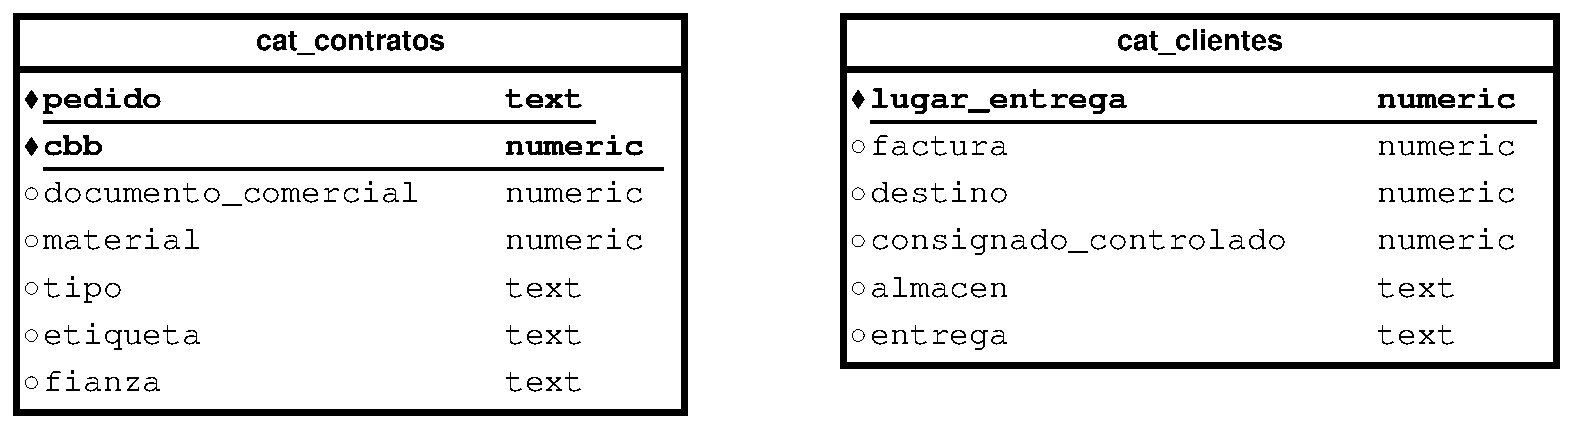
\includegraphics[scale=0.5]{dia-er-reportes} 
  \caption{Diagrama Entidad Relación de los catálogos para la generación de vistas.}
  \label{fig:dia-er-reportes}
\end{figure}
\paragraph{cat{\textunderscore}clientes:} este catálogo contiene información sobre la localización física de los lugares donde deben ser entregados los productos.
\paragraph{cat{\textunderscore}contratos:} este catálogo contiene información sobre acuerdos comerciales referentes a los productos requeridos en las órdenes de reposición.


\section{Resumen}
En este capítulo se ha mostrado la arquitectura del Sistema AutoSA, los componentes del mismo y las interfaces que ofrecen. Posteriormente se ha mostrado el flujo de mensajes entre los componentes del sistema para llevar a cabo los casos de uso del Capítulo \ref{cap2}. Asimismo se ha modelado la base de datos que a grandes rasgos está destinada a almacenar información de las órdenes de reposición e información de los usuarios del Sistema AutoSA.\\
El diseño planteado será implementado en el siguiente capítulo, donde se verá a detalle el funcionamiento de cada módulo, así como algoritmos, tecnologías y marcos de trabajo utilizados. 